\chapter{อาร์เรย์{\wbr}และ{\wbr}พอยน์เตอร์}
\label{chapter:arrays}

ใน{\wbr}บท{\wbr}นี้{\wbr}เรา{\wbr}จะ{\wbr}พิจารณา{\wbr}โครงสร้าง{\wbr}ข้อมูล{\wbr}พื้นฐาน{\wbr}สำหรับ{\wbr}จัด{\wbr}เก็บ{\wbr}และ{\wbr}ประมวลผล{\wbr}ข้อมูล{\wbr}จำนวน{\wbr}มาก{\wbr}ที่{\wbr}เรียก{\wbr}ว่า{\em
  อาร์เรย์} (array) รวม{\wbr}ไป{\wbr}ถึง{\wbr}ข้อมูล{\wbr}ประเภท{\em พอยน์เตอร์} (pointer)
ซึ่ง{\wbr}เก็บ{\wbr}ตำแหน่ง{\wbr}ภายใน{\wbr}หน่วยความจำ{\wbr}
โดย{\wbr}เรา{\wbr}จะ{\wbr}เริ่ม{\wbr}พิจารณา{\wbr}แนว{\wbr}คิด{\wbr}ของ{\wbr}โครงสร้าง{\wbr}ข้อมูล{\wbr}และ{\wbr}ชนิด{\wbr}ข้อมูล{\wbr}ดังกล่าว{\wbr}โดย{\wbr}ไม่{\wbr}ขึ้น{\wbr}กับ{\wbr}ภาษา{\wbr}โปรแกรม{\wbr}ที่{\wbr}ใช้{\wbr}
จากนั้น{\wbr}เรา{\wbr}จะ{\wbr}ศึกษา{\wbr}วิธีการ{\wbr}เขียน{\wbr}ใน{\wbr}ภาษา C++
และ{\wbr}ศึกษา{\wbr}ความ{\wbr}สัมพันธ์{\wbr}ระหว่าง{\wbr}พอยน์เตอร์{\wbr}และ{\wbr}อาร์เรย์{\wbr}ซึ่ง{\wbr}เป็นคุณ{\wbr}ลักษณะ{\wbr}เฉพาะที่{\wbr}มี{\wbr}ใน{\wbr}ภาษา{\wbr}ตระกูล{\wbr}
C และ C++

ใน{\wbr}บท{\wbr}นี้ เรา{\wbr}จะ{\wbr}เริ่ม{\wbr}ศึกษา{\wbr}การ{\wbr}วิเคราะห์{\wbr}เวลา{\wbr}การ{\wbr}ทำงาน{\wbr}ของ{\wbr}อัล{\wbr}กอ{\wbr}ริ{\wbr}ทึม{\wbr}อย่าง{\wbr}ง่าย ก่อน{\wbr}ที่{\wbr}จะ{\wbr}ไป{\wbr}พิจารณา{\wbr}อย่าง{\wbr}เป็นทางการ{\wbr}ใน{\wbr}บท{\wbr}ที่~\ref{chapter:analysis}

\section{อาร์เรย์}
อาร์เรย์เป็น{\wbr}โครงสร้าง{\wbr}ข้อมูล{\wbr}ที่{\wbr}เก็บ{\wbr}กลุ่ม{\wbr}ของ{\wbr}ข้อมูล{\wbr}เป็น{\wbr}รายการ{\wbr}
โดย{\wbr}ที่{\wbr}ข้อมูล{\wbr}แต่ละ{\wbr}ตัว{\wbr}จะ{\wbr}ถูก{\wbr}เก็บ{\wbr}ต่อเนื่อง{\wbr}กัน{\wbr}ใน{\wbr}หน่วยความจำ และ{\wbr}ถูก{\wbr}อ้าง{\wbr}ถึง{\wbr}โดย{\wbr}ใช้{\wbr}ดัชนี (index)
ตัวอย่าง{\wbr}ง่าย ๆ ของ{\wbr}อาร์เรย์{\wbr}คือ{\wbr}รายการ{\wbr}ข้อมูล{\wbr}ด้าน{\wbr}ล่าง{\wbr}นี้{\wbr}

\begin{center}
2, 3, 5, 7, 11, 13, 17, 19, 23
\end{center}

ถ้า{\wbr}เรา{\wbr}เรียก{\wbr}รายการ{\wbr}ดังกล่าว{\wbr}ว่า{\wbr}รายการ $A$ และ{\wbr}อ้าง{\wbr}ถึง{\wbr}ข้อมูล{\wbr}แต่ละ{\wbr}ตัว{\wbr}ด้วย{\wbr}ดัชนี{\wbr}ที่{\wbr}เริ่มต้น{\wbr}ด้วย 0
ข้อมูล{\wbr}แต่ละ{\wbr}ตัว{\wbr}ใน{\wbr}รายการ{\wbr}จะ{\wbr}ถูก{\wbr}อ้าง{\wbr}ถึง{\wbr}ได้{\wbr}ดัง{\wbr}ตาราง{\wbr}ใน{\wbr}รูป{\wbr}ที่~\ref{fig:array-array-access}

\begin{figure}
\begin{center}
\begin{tabular}{|c|c|c|c|c|c|c|c|c|}
\hline
$A[0]$ & $A[1]$ & $A[2]$ & $A[3]$ & $A[4]$ & $A[5]$ & $A[6]$ & $A[7]$ & $A[8]$ \\
\hline
2 & 3 & 5 & 7 & 11 & 13 & 17 & 19 & 23\\
\hline
\end{tabular}
\end{center}
\caption{การ{\wbr}อ้าง{\wbr}ถึง{\wbr}ข้อมูล{\wbr}แต่ละ{\wbr}ตัว{\wbr}ใน{\wbr}อาร์เรย์ $A$}
\label{fig:array-array-access}
\end{figure}


\begin{quiz}{การ{\wbr}คำนวณ{\wbr}ค่า}
จง{\wbr}หา{\wbr}ผลลัพธ์{\wbr}ของ{\wbr}นิพจน์{\wbr}เหล่านี้ (1) $A[4]$, (2) $A[7]$, (3) $A[A[0]]$, 
(4) $A[A[A[0]]]$, (5) $A[200]$
\end{quiz}
\begin{quizans}
(1) 11, (2) 19, (3) 5, (4) 13, (5) ไม่{\wbr}มี{\wbr}ค่า (ดู{\wbr}อธิบาย{\wbr}เพิ่มเติม)
\end{quizans}

การ{\wbr}หา{\wbr}คำตอบ{\wbr}ของ{\wbr}คำถาม{\wbr}ที่ (3) นั้น จำเป็น{\wbr}ต้อง{\wbr}เข้าใจ{\wbr}ขั้นตอน{\wbr}การ{\wbr}คำนวณ{\wbr}ค่า{\wbr}ของ{\wbr}นิพจน์{\wbr}
เรา{\wbr}ต้องการ{\wbr}หา{\wbr}ค่า $A[A[0]]$ ดังนั้น{\wbr}เรา{\wbr}ต้องหา{\wbr}ค่า $A[0]$ ก่อน{\wbr}
เมื่อ{\wbr}พิจารณา{\wbr}ใน{\wbr}อาร์เรย์{\wbr}เรา{\wbr}พบ{\wbr}ว่า $A[0]$ คือ $2$ ดังนั้น จากนั้น{\wbr}เรา{\wbr}จึง{\wbr}พิจารณา{\wbr}ข้อมูล{\wbr}
$A[2]$ ใน{\wbr}อา{\wbr}รเรย์ ซึ่ง{\wbr}จะ{\wbr}ได้{\wbr}ค่า $5$

ใน{\wbr}การ{\wbr}ทำงาน{\wbr}จริง อาร์เรย์จะ{\wbr}เก็บ{\wbr}ใน{\wbr}หน่วยความจำ{\wbr}ที่{\wbr}ต่อเนื่อง{\wbr}กัน{\wbr}
และ{\wbr}มักจะ{\wbr}มี{\wbr}ขอบเขต{\wbr}ที่{\wbr}จำกัด{\wbr}และ{\wbr}ต้อง{\wbr}ระบุ{\wbr}เมื่อ{\wbr}เริ่ม{\wbr}ใช้ เช่น อาร์เรย์จำนวน 100 ช่อง หรือ{\wbr}
100000 ช่อง{\wbr}เป็นต้น รูป{\wbr}ที่~\ref{fig:array-array-in-mem}
แสดง{\wbr}ตัวอย่าง{\wbr}ของ{\wbr}การ{\wbr}เก็บ{\wbr}ข้อมูล{\wbr}ของ{\wbr}อาร์เรย์{\wbr}ใน{\wbr}หน่วยความจำ{\wbr}

\begin{figure}
TODO: ใส่{\wbr}รูป{\wbr}
\caption{การ{\wbr}เก็บ{\wbr}ข้อมูล{\wbr}ของ{\wbr}อาร์เรย์{\wbr}ใน{\wbr}หน่วยความจำ}
\label{fig:array-array-in-mem}
\end{figure}

คำถาม{\wbr}ที่ (5) เป็น{\wbr}การ{\wbr}อ้าง{\wbr}ถึง{\wbr}ข้อมูล{\wbr}ที่อยู่{\wbr}นอก{\wbr}ขอบเขต{\wbr}ของ{\wbr}อาร์เรย์
ซึ่ง{\wbr}ผลลัพธ์{\wbr}ที่{\wbr}ได้{\wbr}จะ{\wbr}ขึ้น{\wbr}กับ{\wbr}ภาษา{\wbr}โปรแกรม{\wbr}ที่{\wbr}ใช้ สำหรับ{\wbr}ภาษา C หรือ C++
ผลลัพธ์{\wbr}ที่{\wbr}ได้{\wbr}จะ{\wbr}ขึ้น{\wbr}กับ{\wbr}ข้อมูล{\wbr}ใน{\wbr}หน่วยความจำ{\wbr}ใน{\wbr}ตำแหน่ง{\wbr}ที่ $A[200]$ ควร{\wbr}จะ{\wbr}อยู่{\wbr}
เรา{\wbr}จะ{\wbr}ได้{\wbr}ศึกษา{\wbr}รายละเอียด{\wbr}นี้{\wbr}ต่อไป อย่างไรก็ตาม ปกติ{\wbr}แล้ว ใน{\wbr}การ{\wbr}ใช้{\wbr}งาน{\wbr}อาร์เรย์
เรา{\wbr}จะ{\wbr}ไม่{\wbr}อ้าง{\wbr}ถึง{\wbr}ข้อมูล{\wbr}ที่อยู่{\wbr}นอก{\wbr}ขอบเขต{\wbr}ของ{\wbr}อาร์เรย์

การ{\wbr}ระบุ{\wbr}ดัชนี{\wbr}ของ{\wbr}ข้อมูล{\wbr}ใน{\wbr}อาร์เรย์{\wbr}ใน{\wbr}หนังสือ{\wbr}เล่ม{\wbr}นี้{\wbr}จะ{\wbr}อ้างอิง{\wbr}จาก{\wbr}ภาษา{\wbr}ตระกูล{\wbr}ภาษา C
นั่น{\wbr}คือ{\wbr}เริ่มต้น{\wbr}ที่ 0 \ \ สำหรับ{\wbr}บาง{\wbr}ภาษา เรา{\wbr}สามารถ{\wbr}ระบุ{\wbr}ค่า{\wbr}เริ่มต้น{\wbr}ของ{\wbr}ดัชนี{\wbr}ได้{\wbr}และ{\wbr}มัก{\wbr}เริ่ม{\wbr}ที่ 1
เช่น{\wbr}ภาษา{\wbr}ปา{\wbr}ส{\wbr}คา{\wbr}ล (Pascal) เป็นต้น{\wbr}
อย่างไรก็ตาม{\wbr}แนว{\wbr}คิด{\wbr}ใน{\wbr}การ{\wbr}พัฒนา{\wbr}โปรแกรม{\wbr}นั้น{\wbr}จะ{\wbr}ไม่{\wbr}ต่าง{\wbr}กัน{\wbr}

เมื่อ{\wbr}เรา{\wbr}สามารถ{\wbr}อ้าง{\wbr}ถึง{\wbr}ข้อมูล{\wbr}ได้{\wbr}ด้วย{\wbr}ดัชนี{\wbr}
เรา{\wbr}สามารถ{\wbr}ใช้{\wbr}ตัวแปร{\wbr}เพื่อ{\wbr}แทน{\wbr}ค่า{\wbr}ดัชนี{\wbr}ของ{\wbr}ข้อมูล{\wbr}ที่{\wbr}เรา{\wbr}ต้องการ{\wbr}ใช้{\wbr}งาน{\wbr}ได้{\wbr}
ความ{\wbr}สามารถ{\wbr}นี้{\wbr}ทำ{\wbr}ให้{\wbr}เรา{\wbr}สามารถ{\wbr}เขียน{\wbr}โปรแกรม{\wbr}ที่{\wbr}มี{\wbr}ลักษณะ{\wbr}ดัง{\wbr}ด้าน{\wbr}ล่าง{\wbr}ได้{\wbr}

\begin{algt}
\label{alg:array-sum1}
\noindent \hspace*{0.2in} ให้ $x\leftarrow 0$\\
\hspace*{0.2in} พิจารณา ตัวแปร $i\leftarrow 0,1,\ldots,8$\\
\hspace*{0.2in}\hspace*{0.2in} ให้ $x \leftarrow x + A[i]$
\end{algt}

\begin{quiz}{}
อัล{\wbr}กอ{\wbr}ริ{\wbr}ทึม{\wbr}ดังกล่าว{\wbr}คำนวณ{\wbr}ค่า{\wbr}บาง{\wbr}อย่าง{\wbr}ใน{\wbr}ตัวแปร $x$ ค่า{\wbr}นั้น{\wbr}คือ{\wbr}อะไร?
\end{quiz}
\begin{quizans}
ผลรวม{\wbr}ของ{\wbr}ข้อมูล{\wbr}ทั้งหมด{\wbr}ใน{\wbr}อาร์เรย์ $A$
\end{quizans}

สังเกต{\wbr}ว่า{\wbr}อัล{\wbr}กอ{\wbr}ริ{\wbr}ทึม~\ref{alg:array-sum1} เขียน{\wbr}ให้{\wbr}ทำงาน{\wbr}กับ{\wbr}อาร์เรย์ $A$
ที่{\wbr}มี{\wbr}ดัชนี{\wbr}มาก{\wbr}ที่สุด{\wbr}คือ 8 เท่านั้น ใน{\wbr}การ{\wbr}พัฒนา{\wbr}อัล{\wbr}กอ{\wbr}ริ{\wbr}ทึม{\wbr}ทั่วไป{\wbr}เรา{\wbr}มัก{\wbr}เขียน{\wbr}ให้{\wbr}ทำงาน{\wbr}ได้{\wbr}กับ{\wbr}ข้อมูล{\wbr}ทั่วไป{\wbr}
ซึ่ง{\wbr}ใน{\wbr}กรณี{\wbr}นี้ การ{\wbr}จะ{\wbr}ปรับ{\wbr}ให้{\wbr}ทำงาน{\wbr}ได้{\wbr}กับ{\wbr}อาร์เรย์{\wbr}ใด ๆ เรา{\wbr}จะ{\wbr}ต้อง{\wbr}ระบุ{\wbr}ขนาด{\wbr}ของ{\wbr}อาร์เรย์{\wbr}ด้วย{\wbr}
เรา{\wbr}สามารถ{\wbr}เขียน{\wbr}อัล{\wbr}กอ{\wbr}ริ{\wbr}ทึม{\wbr}ดังกล่าว{\wbr}โดย{\wbr}ระบุ{\wbr}พารามิเตอร์{\wbr}ให้{\wbr}ชัดเจน{\wbr}ขึ้น{\wbr}ได้{\wbr}ดัง{\wbr}ด้าน{\wbr}ล่าง{\wbr}

\begin{algt}
\label{alg:array-sum2}
\noindent {\bf คำนวณ{\wbr}ค่า{\wbr}บาง{\wbr}อย่าง{\wbr}ของ{\wbr}อาร์เรย์ $A$ ที่{\wbr}มี{\wbr}ข้อมูล{\wbr}จำนวน $n$ ตัว}\\
\hspace*{0.2in} ให้ $x\leftarrow 0$\\
\hspace*{0.2in} พิจารณา ตัวแปร $i\leftarrow 0,1,\ldots,n-1$\\
\hspace*{0.2in}\hspace*{0.2in} ให้ $x \leftarrow x + A[i]$\\
\hspace*{0.2in} คืน{\wbr}ค่า $x$ เป็น{\wbr}คำตอบ{\wbr}
\end{algt}

\subsection{เวลา{\wbr}ที่{\wbr}ใช้{\wbr}ใน{\wbr}การ{\wbr}ทำงาน}

ค่า{\wbr}พารามิเตอร์ $n$ ที่{\wbr}เรา{\wbr}ส่ง{\wbr}ให้{\wbr}กับ{\wbr}โปรแกรมย่อย ระบุ{\wbr}จำนวน{\wbr}รอบ{\wbr}ของ{\wbr}การ{\wbr}ทำงาน{\wbr}
ซึ่ง{\wbr}จะ{\wbr}เป็น{\wbr}ตัวกำหนด{\wbr}เวลา{\wbr}ที่{\wbr}โปรแกรมย่อย{\wbr}ใช้{\wbr}ใน{\wbr}การ{\wbr}ทำงาน{\wbr}ด้วย อย่างไรก็ตาม{\wbr}
เพียงแค่{\wbr}พิจารณา{\wbr}โปรแกรมย่อย{\wbr}ดังกล่าว เรา{\wbr}ไม่{\wbr}สามารถ{\wbr}ระบุ{\wbr}เวลาจริง ๆ
ที่{\wbr}โปรแกรมย่อย{\wbr}จะ{\wbr}ทำงาน{\wbr}ได้{\wbr}เนื่องจาก{\wbr}เรา{\wbr}ไม่{\wbr}ทราบ{\wbr}ปัจจัย{\wbr}หลาย ๆ อย่าง{\wbr}

\begin{quiz}{เวลา{\wbr}การ{\wbr}ทำงาน{\wbr}จริง{\wbr}บน{\wbr}คอมพิวเตอร์}
ปัจจัย{\wbr}อะไร{\wbr}บ้าง{\wbr}ที่{\wbr}กำหนด{\wbr}เวลา{\wbr}ทำงาน{\wbr}บน{\wbr}คอมพิวเตอร์{\wbr}จริง ๆ ของ{\wbr}โปรแกรมย่อย{\wbr}ข้างต้น{\wbr}
\end{quiz}
\begin{quizans}
เวลา{\wbr}ใน{\wbr}การ{\wbr}ทำงาน{\wbr}จริง ขึ้น{\wbr}กับ (1) โปรแกรม{\wbr}ภาษาคอมพิวเตอร์{\wbr}ที่{\wbr}เขียน{\wbr}จาก{\wbr}โปรแกรมย่อย (2)
คอม{\wbr}ไพ{\wbr}เลอร์{\wbr}ที่{\wbr}ใช้ (3) เครื่อง{\wbr}คอมพิวเตอร์{\wbr}ที่{\wbr}นำ{\wbr}โปรแกรม{\wbr}ไป{\wbr}ทำงาน{\wbr}
และ{\wbr}สถานะ{\wbr}ของ{\wbr}เครื่องใน{\wbr}ขณะที่{\wbr}โปรแกรม{\wbr}ทำงาน  
\end{quizans}

สังเกต{\wbr}ว่า{\wbr}การ{\wbr}พิจารณา{\wbr}แค่{\wbr}อัล{\wbr}กอ{\wbr}ริ{\wbr}ทึม{\wbr}เพียง{\wbr}อย่างเดียว{\wbr}
หรือ{\wbr}กระทั่ง{\wbr}จะ{\wbr}พิจารณา{\wbr}โปรแกรม{\wbr}ใน{\wbr}ภาษาเครื่อง{\wbr}ที่{\wbr}ถูก{\wbr}คอมไพล์{\wbr}แล้ว{\wbr}ร่วม{\wbr}ด้วย{\wbr}
ก็{\wbr}ไม่{\wbr}สามารถ{\wbr}ทำ{\wbr}ให้{\wbr}เรา{\wbr}ระบุ{\wbr}เวลา{\wbr}การ{\wbr}ทำงาน{\wbr}บน{\wbr}คอมพิวเตอร์{\wbr}จริง{\wbr}ได้{\wbr}อย่าง{\wbr}แม่นยำ{\wbr}
ยิ่ง{\wbr}ใน{\wbr}ปัจจุบัน{\wbr}ที่{\wbr}คอมพิวเตอร์{\wbr}สามารถ{\wbr}ทำงาน{\wbr}หลาย ๆ งาน{\wbr}ใน{\wbr}เวลา{\wbr}เดียวกัน{\wbr}
การ{\wbr}ทำนาย{\wbr}เวลา{\wbr}การ{\wbr}ทำงาน{\wbr}จริง{\wbr}ยิ่ง{\wbr}กระทำ{\wbr}ได้{\wbr}ยาก{\wbr}ขึ้น{\wbr}ด้วย{\wbr}

อย่างไรก็ตาม แม้{\wbr}การ{\wbr}ระบุ{\wbr}เวลา{\wbr}การ{\wbr}ทำงาน{\wbr}จริง ๆ ทำ{\wbr}ได้{\wbr}ยาก{\wbr}
การ{\wbr}ทำนาย{\wbr}เวลา{\wbr}การ{\wbr}ทำงาน{\wbr}ของ{\wbr}อัล{\wbr}กอ{\wbr}ริ{\wbr}ทึม{\wbr}ก่อน{\wbr}ที่{\wbr}จะ{\wbr}นำ{\wbr}ไป{\wbr}พัฒนา{\wbr}เป็น{\wbr}โปรแกรม{\wbr}ก็{\wbr}ยัง{\wbr}เป็น{\wbr}สิ่ง{\wbr}จำเป็น{\wbr}มาก{\wbr}
เนื่องจาก{\wbr}ใน{\wbr}หลาย ๆ เรา{\wbr}สามารถ{\wbr}เลือก{\wbr}ใช้{\wbr}อัล{\wbr}กอ{\wbr}ริ{\wbr}ทึม{\wbr}ได้{\wbr}หลากหลาย{\wbr}
และ{\wbr}อัล{\wbr}กอ{\wbr}ริ{\wbr}ทึม{\wbr}เหล่านั้น{\wbr}ก็{\wbr}มี{\wbr}ความ{\wbr}ซับซ้อน{\wbr}ใน{\wbr}การ{\wbr}นำ{\wbr}ไป{\wbr}พัฒนา{\wbr}เป็น{\wbr}โปรแกรม{\wbr}ที่{\wbr}แตกต่าง{\wbr}กัน{\wbr}
โปรแกรมเมอร์{\wbr}จึง{\wbr}ต้อง{\wbr}เลือก{\wbr}ใช้{\wbr}อัล{\wbr}กอ{\wbr}ริ{\wbr}ทึม{\wbr}ให้{\wbr}เหมาะสม นั่น{\wbr}คือ{\wbr}เป็น{\wbr}อัล{\wbr}กอ{\wbr}ริ{\wbr}ทึม{\wbr}ที่{\wbr}เมื่อ{\wbr}นำ{\wbr}ไป{\wbr}พัฒนา{\wbr}แล้ว{\wbr}
มี{\wbr}ประสิทธิภาพ{\wbr}พอ (ทำงาน{\wbr}ได้{\wbr}ทัน{\wbr}เวลา)
และ{\wbr}มี{\wbr}ความ{\wbr}ซับซ้อน{\wbr}ใน{\wbr}การ{\wbr}เขียน{\wbr}ใน{\wbr}ระดับ{\wbr}ที่{\wbr}โปรแกรมเมอร์{\wbr}สามารถ{\wbr}จัดการ{\wbr}ได้{\wbr}
การ{\wbr}เลือก{\wbr}นำ{\wbr}อัล{\wbr}กอ{\wbr}ริ{\wbr}ทึม{\wbr}ที่{\wbr}ทราบ{\wbr}ว่า{\wbr}มี{\wbr}ประสิทธิภาพ{\wbr}ดี{\wbr}ที่สุด{\wbr}ไป{\wbr}พัฒนา{\wbr}นั้น{\wbr}
อาจ{\wbr}ไม่{\wbr}ใช่{\wbr}ทางเลือก{\wbr}ที่{\wbr}ดี{\wbr}ที่สุด{\wbr}ก็{\wbr}เป็น{\wbr}ได้{\wbr}

ดังนั้น เรา{\wbr}จะ{\wbr}พยายาม{\wbr}วิเคราะห์{\wbr}เวลา{\wbr}การ{\wbr}ทำงาน{\wbr}ของ{\wbr}โปรแกรมย่อย{\wbr}
ที่อยู่{\wbr}ใน{\wbr}รูป{\wbr}ของ{\wbr}โปรแกรม{\wbr}ลำ{\wbr}ลอง{\wbr}ด้าน{\wbr}บน ให้{\wbr}ละเอียด{\wbr}เท่า{\wbr}ที่{\wbr}เรา{\wbr}พอจะ{\wbr}ทำ{\wbr}ได้{\wbr}
แน่นอน{\wbr}เรา{\wbr}จำเป็น{\wbr}ต้อง{\wbr}เพิ่ม{\wbr}ข้อสมมติ{\wbr}หลาย{\wbr}อย่าง{\wbr}เพื่อให้{\wbr}การ{\wbr}วิเคราะห์{\wbr}เป็น{\wbr}ไป{\wbr}ได้{\wbr}

ข้อสมมติ{\wbr}ข้อ{\wbr}แรก (ที่{\wbr}เรา{\wbr}จะ{\wbr}ใช้{\wbr}ตลอด{\wbr}ใน{\wbr}หนังสือ{\wbr}เล่ม{\wbr}นี้) คือ{\wbr}
เรา{\wbr}จะ{\wbr}สมมติ{\wbr}ว่า{\wbr}คอมพิวเตอร์{\wbr}นั้น{\wbr}ทำงาน{\wbr}ทีละ{\wbr}คำสั่ง นั่น{\wbr}คือ{\wbr}ไม่{\wbr}ใช่{\wbr}คอมพิวเตอร์{\wbr}แบบ{\wbr}ขนาน{\wbr}
หรือ{\wbr}เป็น{\wbr}คอมพิวเตอร์{\wbr}ที่{\wbr}มี{\wbr}หน่วย{\wbr}ประมวลผล{\wbr}หลาย{\wbr}ตัว{\wbr}ทำงาน{\wbr}พร้อมกัน\footnote{TODO:
  ระบุ{\wbr}ว่า{\wbr}ถึง{\wbr}จะ{\wbr}เป็น{\wbr}กรณี{\wbr}ดังกล่าว การ{\wbr}วิเคราะห์{\wbr}ก็{\wbr}ยัง{\wbr}เป็น{\wbr}ไป{\wbr}ได้}

ถ้า{\wbr}พิจารณา{\wbr}ต่อไป เรา{\wbr}จะ{\wbr}พบ{\wbr}ว่า{\wbr}โปรแกรมย่อย~\ref{alg:array-sum2}
ทำงาน{\wbr}โดย{\wbr}ใช้เวลา{\wbr}ใน{\wbr}การ{\wbr}ทำงาน{\wbr}ที่{\wbr}แปรผัน{\wbr}ตาม{\wbr}ค่า{\wbr}พารามิเตอร์ $n$
เพื่อ{\wbr}จะ{\wbr}ให้{\wbr}เรา{\wbr}สามารถ{\wbr}วิเคราะห์{\wbr}เวลา{\wbr}การ{\wbr}ทำงาน{\wbr}ออก{\wbr}มา{\wbr}ได้{\wbr}
เรา{\wbr}จะ{\wbr}สมมติ{\wbr}ว่า{\wbr}คอมพิวเตอร์{\wbr}เมื่อ{\wbr}ทำงาน{\wbr}ตาม{\wbr}โปรแกรม{\wbr}ดังกล่าว ใช้เวลา 1
หน่วย{\wbr}ใน{\wbr}การ{\wbr}ประมวลผล{\wbr}คำสั่ง{\wbr}แต่ละ{\wbr}บรรทัด{\wbr}
เรา{\wbr}จะ{\wbr}สามารถ{\wbr}คำนวณ{\wbr}เวลา{\wbr}ที่{\wbr}โปรแกรม{\wbr}ดังกล่าว{\wbr}ใช้{\wbr}โดย{\wbr}พิจารณา{\wbr}จำนวน{\wbr}ครั้ง{\wbr}ที่{\wbr}คำสั่ง{\wbr}ใน{\wbr}แต่ละ{\wbr}บรรทัด{\wbr}ทำงาน{\wbr}
ดัง{\wbr}ด้าน{\wbr}ล่าง{\wbr}

\begin{algt}
\noindent \hspace*{0.2in} ให้ $x\leftarrow 0$   \ \ \ \ $\rhd\rhd\rhd$ ทำงาน 1 ครั้ง\\
\hspace*{0.2in} พิจารณา ตัวแปร $i\leftarrow 0,1,\ldots,n-1$  \ \ \ \ $\rhd\rhd\rhd$ ทำงาน $n$ ครั้ง\\
\hspace*{0.2in}\hspace*{0.2in} ให้ $x \leftarrow x + A[i]$  \ \ \ \ $\rhd\rhd\rhd$ ทำงาน $n$ ครั้ง\\
\hspace*{0.2in} คืน{\wbr}ค่า $x$ เป็น{\wbr}คำตอบ  \ \ \ \ $\rhd\rhd\rhd$ ทำงาน 1 ครั้ง{\wbr}
\end{algt}

ดังนั้น{\wbr}เรา{\wbr}จะ{\wbr}ได้{\wbr}ว่า{\wbr}เวลา{\wbr}รวม{\wbr}คือ $2n + 2$ หน่วย คำถาม{\wbr}ที่{\wbr}ตาม{\wbr}มา{\wbr}ก็{\wbr}คือ{\wbr}
ผลลัพธ์{\wbr}จาก{\wbr}การ{\wbr}วิเคราะห์{\wbr}ดังกล่าว{\wbr}มี{\wbr}ความ{\wbr}แม่นยำ{\wbr}
และ{\wbr}สามารถ{\wbr}นำ{\wbr}ไป{\wbr}ใช้{\wbr}วิเคราะห์{\wbr}และ{\wbr}ตัดสินใจ{\wbr}ต่อไป{\wbr}ได้{\wbr}เพียงใด{\wbr}
เรา{\wbr}จะ{\wbr}พิจารณา{\wbr}ผล{\wbr}จาก{\wbr}การ{\wbr}สมมติ{\wbr}และ{\wbr}ความ{\wbr}ถูกต้อง{\wbr}ที่{\wbr}ใช้ได้{\wbr}ใน{\wbr}บท{\wbr}ที่~\ref{chapter:analysis}

\subsection{การ{\wbr}ประมวลผล{\wbr}รายการ{\wbr}ด้วย{\wbr}อาร์เรย์}
\label{sect:array-list-processing}

ใน{\wbr}ส่วน{\wbr}นี้{\wbr}เรา{\wbr}จะ{\wbr}พัฒนา{\wbr}โปรแกรม{\wbr}ลำ{\wbr}ลอง{\wbr}เพื่อ{\wbr}ประมวลผล{\wbr}ข้อมูล{\wbr}ใน{\wbr}รายการ{\wbr}ที่{\wbr}เก็บ{\wbr}ใน{\wbr}อาร์เรย์
พร้อมกับ{\wbr}วิเคราะห์{\wbr}เวลา{\wbr}การ{\wbr}ทำงาน{\wbr}

\begin{quiz}{}
สมมติ{\wbr}ว่า{\wbr}เรา{\wbr}มี{\wbr}รายการ{\wbr}ของ{\wbr}ข้อมูล ลอง{\wbr}นึก{\wbr}ตัวอย่าง{\wbr}การ{\wbr}ประมวลผล{\wbr}ที่{\wbr}เรา{\wbr}สามารถ{\wbr}กระทำ{\wbr}กับ{\wbr}ข้อมูล{\wbr}ใน{\wbr}รายการ{\wbr}นี้{\wbr}
\end{quiz}

ก่อน{\wbr}ที่{\wbr}เรา{\wbr}จะ{\wbr}ประมวลผล{\wbr}ได้ เรา{\wbr}ต้อง{\wbr}พิจารณา{\wbr}วิธีการ{\wbr}จัด{\wbr}เก็บ{\wbr}ข้อมูล{\wbr}แบบ{\wbr}รายการ{\wbr}ลง{\wbr}ใน{\wbr}อาร์เรย์{\wbr}ก่อน{\wbr}
สังเกต{\wbr}ว่า{\wbr}โครงสร้าง{\wbr}ข้อมูล{\wbr}แบบ{\wbr}อาร์เรย์{\wbr}มี{\wbr}ลักษณะ{\wbr}เป็น{\wbr}รายการ{\wbr}อยู่{\wbr}แล้ว{\wbr}
อย่างไรก็ตาม{\wbr}ใน{\wbr}การ{\wbr}จัดการ{\wbr}กับ{\wbr}รายการ{\wbr}ที่{\wbr}มี{\wbr}จำนวน{\wbr}ข้อมูล{\wbr}เปลี่ยนแปลง{\wbr}ได้{\wbr}
การ{\wbr}ใช้{\wbr}อาร์เรย์{\wbr}เพียง{\wbr}อย่างเดียว{\wbr}นั้น{\wbr}ไม่{\wbr}เพียงพอ{\wbr}

\begin{quiz}{}
อะไร{\wbr}คือ{\wbr}สิ่ง{\wbr}ที่{\wbr}ขาด{\wbr}หาย{\wbr}ไป ถ้า{\wbr}เรา{\wbr}ใช้{\wbr}แค่{\wbr}อาร์เรย์{\wbr}ใน{\wbr}การ{\wbr}จัด{\wbr}เก็บ{\wbr}รายการ{\wbr}ที่{\wbr}จำนวน{\wbr}ข้อมูล{\wbr}ใน{\wbr}รายการ{\wbr}เปลี่ยนแปลง{\wbr}ได้{\wbr}
\end{quiz}

ดังนั้น เรา{\wbr}จะ{\wbr}ใช้{\wbr}ตัวแปร{\wbr}อีก{\wbr}หนึ่ง{\wbr}ตัว{\wbr}ใน{\wbr}การ{\wbr}เก็บ{\wbr}จำนวน{\wbr}ข้อมูล{\wbr}ที่{\wbr}มี{\wbr}ใน{\wbr}อาร์เรย์
โปรแกรม{\wbr}ลำ{\wbr}ลอง{\wbr}ที่{\wbr}เรา{\wbr}จะ{\wbr}พัฒนา{\wbr}จะ{\wbr}เปลี่ยน{\wbr}ค่า{\wbr}ของ{\wbr}ตัวแปร{\wbr}นี้{\wbr}โดย{\wbr}ตรง{\wbr}เพื่อ{\wbr}ปรับ{\wbr}ให้{\wbr}มี{\wbr}ค่า{\wbr}ที่{\wbr}ถูกต้อง{\wbr}ภายหลัง{\wbr}การ{\wbr}ประมวลผล{\wbr}
ใน{\wbr}การ{\wbr}พัฒนา{\wbr}โปรแกรม{\wbr}ลำ{\wbr}ลอง{\wbr}ให้{\wbr}เป็น{\wbr}โปรแกรม{\wbr}ภาษา C++
การ{\wbr}ทำงาน{\wbr}ดังกล่าว{\wbr}จะ{\wbr}ต้อง{\wbr}ใช้{\wbr}การ{\wbr}ส่ง{\wbr}รับ{\wbr}พารามิเตอร์{\wbr}เป็น{\wbr}พอยน์เตอร์{\wbr}หรือ{\wbr}ส่ง{\wbr}แบบ pass by
reference ซึ่ง{\wbr}เรา{\wbr}จะ{\wbr}ได้{\wbr}พิจารณา{\wbr}ใน{\wbr}ส่วน~\ref{sect:array-pointer-c}
นอกจากนี้{\wbr}ใน{\wbr}บท{\wbr}ที่~\ref{chapter:classes} เรา{\wbr}จะ{\wbr}ได้{\wbr}ศึกษา{\wbr}วิธีการ{\wbr}ที่{\wbr}จะ ``ประกอบ{\wbr}รวม''
อาร์เรย์และ{\wbr}ตัวแปร{\wbr}ที่{\wbr}เก็บ{\wbr}จำนวน{\wbr}ข้อมูล{\wbr}ที่อยู่{\wbr}ใน{\wbr}อาร์เรย์{\wbr}เข้า{\wbr}ด้วย{\wbr}กัน{\wbr}
เพื่อ{\wbr}สร้าง{\wbr}เป็น{\wbr}ชนิด{\wbr}ข้อมูล{\wbr}ใหม่{\wbr}ที่{\wbr}นำ{\wbr}ไป{\wbr}ใช้{\wbr}งาน{\wbr}ได้{\wbr}สะดวก{\wbr}ต่อไป{\wbr}

เรา{\wbr}จะ{\wbr}พิจารณา{\wbr}การ{\wbr}ประมวลผล{\wbr}กับ{\wbr}อาร์เรย์{\wbr}ใน{\wbr}รูปแบบ{\wbr}ต่าง ๆ ดังนี้ (1) การ{\wbr}ค้น{\wbr}ข้อมูล{\wbr}ใน{\wbr}รายการ, (2) การ{\wbr}เพิ่ม{\wbr}ข้อมูล{\wbr}ลง{\wbr}ไป{\wbr}ตอน{\wbr}ท้าย{\wbr}ของ{\wbr}รายการ, (3) การ{\wbr}ลบ{\wbr}ข้อมูล{\wbr}ใน{\wbr}รายการ, และ (4) การ{\wbr}แทรก{\wbr}ข้อมูล{\wbr}ใน{\wbr}รายการ{\wbr}

\subsubsection{การ{\wbr}ค้น{\wbr}ข้อมูล} 
สำหรับ{\wbr}การ{\wbr}ค้น{\wbr}ข้อมูล{\wbr}ใน{\wbr}รายการ{\wbr}
เป้าหมาย{\wbr}ของ{\wbr}การ{\wbr}ทำงาน{\wbr}คือ{\wbr}ทราบ{\wbr}ว่า{\wbr}มี{\wbr}ข้อมูล{\wbr}ที่{\wbr}เรา{\wbr}ต้องการ{\wbr}หา{\wbr}หรือ{\wbr}ไม่ และ{\wbr}ถ้า{\wbr}มี{\wbr}อยู่{\wbr}ที่{\wbr}ตำแหน่ง{\wbr}ใด{\wbr}
ใน{\wbr}กรณี{\wbr}นี้{\wbr}เรา{\wbr}จะ{\wbr}ต้อง{\wbr}พิจารณา{\wbr}ข้อมูล{\wbr}ทุก{\wbr}ตัว{\wbr}ใน{\wbr}รายการ{\wbr}
โปรแกรม{\wbr}ลำ{\wbr}ลอง{\wbr}มี{\wbr}ลักษณะ{\wbr}ไม่{\wbr}ต่าง{\wbr}จาก{\wbr}ที่{\wbr}เรา{\wbr}เคย{\wbr}เขียน{\wbr}เท่าใด{\wbr}นัก{\wbr}

\begin{algt}
\noindent {\bf ค้นหา{\wbr}ข้อมูล $x$ ใน{\wbr}อาร์เรย์ $A$ ที่{\wbr}มี{\wbr}ข้อมูล{\wbr}จำนวน $n$ ตัว}\\
\hspace*{0.2in} พิจารณา ตัวแปร $i\leftarrow 0,1,\ldots, n-1$\\
\hspace*{0.2in}\hspace*{0.2in} ถ้า $A[i] = x$\\
\hspace*{0.2in}\hspace*{0.2in}\hspace*{0.2in} คืน{\wbr}ค่า $i$ เป็น{\wbr}ผลลัพธ์\\
\hspace*{0.2in} ตอบ{\wbr}ว่า{\wbr}ไม่{\wbr}พบ{\wbr}ค่า{\wbr}ที่{\wbr}ต้องการ{\wbr}
\end{algt}

ใน{\wbr}การ{\wbr}พัฒนา{\wbr}โปรแกรม{\wbr}จริง ๆ
เรา{\wbr}จะ{\wbr}ต้อง{\wbr}จัดการ{\wbr}ใน{\wbr}กรณี{\wbr}ที่{\wbr}จะ{\wbr}ต้อง{\wbr}ตอบ{\wbr}ว่า{\wbr}ไม่{\wbr}พบ{\wbr}ค่า{\wbr}ที่{\wbr}ต้องการ{\wbr}ให้{\wbr}ชัดเจน{\wbr}กว่า{\wbr}นี้{\wbr}
แต่{\wbr}ใน{\wbr}ขณะนี้{\wbr}เรา{\wbr}จะ{\wbr}สมมติ{\wbr}ว่า{\wbr}โปรแกรมย่อย{\wbr}สามารถ{\wbr}ตอบ{\wbr}แบบ{\wbr}นี้{\wbr}ได้{\wbr}

\begin{quiz}{}
ใน{\wbr}กรณี{\wbr}ของ{\wbr}โปรแกรมย่อย{\wbr}สำหรับ{\wbr}หา{\wbr}ผลรวม เรา{\wbr}พบ{\wbr}ว่า{\wbr}โปรแกรม{\wbr}ทำงาน{\wbr}ใน{\wbr}เวลา{\wbr}ที่{\wbr}แปรผัน{\wbr}กับ{\wbr}ค่า $n$
เสมอ เป็น{\wbr}ไป{\wbr}ได้{\wbr}หรือ{\wbr}ไม่ ที่{\wbr}โปรแกรมย่อย{\wbr}สำหรับ{\wbr}จะ{\wbr}ทำงาน{\wbr}โดย{\wbr}วน{\wbr}รอบ{\wbr}เป็น{\wbr}จำนวน{\wbr}ครั้ง{\wbr}ที่{\wbr}น้อย{\wbr}กว่า{\wbr}ค่า $n$ มาก? และ{\wbr}เป็น{\wbr}ใน{\wbr}กรณี{\wbr}ใด?
\end{quiz}

\begin{quiz}{}
สำหรับ{\wbr}อาร์เรย์{\wbr}ที่{\wbr}มี{\wbr}ข้อมูล $n$ ตัว เมื่อใด{\wbr}ที่{\wbr}โปรแกรมย่อย{\wbr}จะ{\wbr}ทำงาน{\wbr}โดย{\wbr}วน{\wbr}รอบ{\wbr}มาก{\wbr}ที่สุด{\wbr}
\end{quiz}

โปรแกรมย่อย{\wbr}ข้างต้น{\wbr}อาจ{\wbr}จะ{\wbr}ทำงาน{\wbr}ได้{\wbr}รวดเร็ว{\wbr}มาก ถ้า{\wbr}ข้อมูล{\wbr}ที่{\wbr}ต้องการ{\wbr}ค้นหา{\wbr}อยู่{\wbr}ตอน{\wbr}ต้น{\wbr}ของ{\wbr}อาร์เรย์
โปรแกรมย่อย{\wbr}ลักษณะ{\wbr}นี้{\wbr}เป็น{\wbr}ตัวอย่าง{\wbr}ที่{\wbr}ดี{\wbr}ของ{\wbr}โปรแกรมย่อย{\wbr}ที่{\wbr}เวลา{\wbr}การ{\wbr}ทำงาน{\wbr}ขึ้น{\wbr}กับ{\wbr}ข้อมูล{\wbr}ป้อน{\wbr}เข้า{\wbr}
ทำ{\wbr}ให้{\wbr}ใน{\wbr}การ{\wbr}วิเคราะห์{\wbr}เวลา{\wbr}การ{\wbr}ทำงาน{\wbr}นั้น เรา{\wbr}จำเป็น{\wbr}จะ{\wbr}ต้อง{\wbr}พิจารณา{\wbr}ข้อมูล{\wbr}ป้อน{\wbr}เข้า{\wbr}ด้วย{\wbr}
อย่างไรก็ตาม{\wbr}เรา{\wbr}ไม่{\wbr}สามารถ{\wbr}ที่{\wbr}จะ{\wbr}วิเคราะห์{\wbr}เวลา{\wbr}การ{\wbr}ทำงาน{\wbr}ของ{\wbr}โปรแกรม{\wbr}ลำ{\wbr}ลอง{\wbr}บน{\wbr}ข้อมูล{\wbr}ป้อน{\wbr}เข้า{\wbr}ทุก{\wbr}รูปแบบ{\wbr}ได้{\wbr}
เพราะว่า{\wbr}จำนวน{\wbr}ของ{\wbr}ข้อมูล{\wbr}ป้อน{\wbr}เข้า{\wbr}นั้น{\wbr}มี{\wbr}ไม่{\wbr}จำกัด{\wbr}

ใน{\wbr}ทาง{\wbr}ปฏิบัติ{\wbr}แล้ว เรา{\wbr}จึง{\wbr}จะ{\wbr}แบ่ง{\wbr}วิเคราะห์{\wbr}เวลา{\wbr}การ{\wbr}ทำงาน{\wbr}เป็น{\wbr}กรณี{\wbr}ย่อย ๆ สาม{\wbr}กรณี{\wbr}คือ{\wbr}
\begin{itemize}
\item การ{\wbr}วิเคราะห์{\wbr}ใน{\wbr}กรณี{\wbr}ที่{\wbr}ดี{\wbr}ที่สุด (best-case analysis),
\item การ{\wbr}วิเคราะห์{\wbr}ใน{\wbr}กรณี{\wbr}ที่{\wbr}เลวร้าย{\wbr}ที่สุด (worst-case analysis), และ{\wbr}
\item การ{\wbr}วิเคราะห์{\wbr}ใน{\wbr}กรณี{\wbr}เฉลี่ย (average-case analysis)
\end{itemize}

สำหรับ{\wbr}การ{\wbr}วิเคราะห์{\wbr}ใน{\wbr}กรณี{\wbr}เฉลี่ย{\wbr}นั้น เป็น{\wbr}การ{\wbr}วิเคราะห์{\wbr}เชิง{\wbr}ความน่าจะเป็น{\wbr}
เรา{\wbr}จำเป็น{\wbr}จะ{\wbr}ต้อง{\wbr}นิยาม{\wbr}ลักษณะ{\wbr}การ{\wbr}กระจาย{\wbr}ของ{\wbr}ข้อมูล{\wbr}ป้อน{\wbr}เข้า{\wbr}ให้{\wbr}ชัดเจน จึง{\wbr}จะ{\wbr}สามารถ{\wbr}กระทำ{\wbr}ได้{\wbr}
เรา{\wbr}จะ{\wbr}ได้{\wbr}ศึกษา{\wbr}ตัวอย่าง{\wbr}การ{\wbr}วิเคราะห์{\wbr}นี้{\wbr}ใน{\wbr}บท{\wbr}ที่~\ref{chapter:analysis} (TODO:
เพิ่ม{\wbr}หรือ{\wbr}ลบ) ใน{\wbr}ที่นี้{\wbr}เรา{\wbr}จะ{\wbr}สนใจ{\wbr}เฉพาะ{\wbr}การ{\wbr}วิเคราะห์{\wbr}กรณี{\wbr}ที่{\wbr}ดี{\wbr}ที่สุด{\wbr}
และ{\wbr}การ{\wbr}วิเคราะห์{\wbr}ใน{\wbr}กรณี{\wbr}ที่{\wbr}เลวร้าย{\wbr}ที่สุด{\wbr}เท่านั้น{\wbr}

กรณี{\wbr}ที่{\wbr}ดี{\wbr}ที่สุด{\wbr}คือ{\wbr}กรณี{\wbr}ที่{\wbr}มี{\wbr}การ{\wbr}วน{\wbr}รอบ{\wbr}เพียง{\wbr}รอบ{\wbr}เดียว นั้น{\wbr}คือ{\wbr}เป็น{\wbr}กรณี{\wbr}ที่ $A[0] = x$
สังเกต{\wbr}ว่า{\wbr}ถ้า{\wbr}เรา{\wbr}สมมติ{\wbr}ให้การ{\wbr}ประมวลผล{\wbr}แต่ละ{\wbr}บรรทัด{\wbr}ใช้เวลา 1 หน่วย ใน{\wbr}กรณี{\wbr}ที่{\wbr}ดี{\wbr}ที่สุด{\wbr}
โปรแกรม{\wbr}ลำ{\wbr}ลอง{\wbr}ดังกล่าว{\wbr}จะ{\wbr}ใช้เวลา{\wbr}ทำงาน $4$ หน่วย{\wbr}

กรณี{\wbr}ที่{\wbr}เลวร้าย{\wbr}ที่สุด{\wbr}เกิด{\wbr}ขึ้น{\wbr}เมื่อ{\wbr}ไม่{\wbr}พบ{\wbr}ข้อมูล{\wbr}ที่{\wbr}ต้องการ{\wbr}หา{\wbr}
สังเกต{\wbr}ว่า{\wbr}โปรแกรม{\wbr}จะ{\wbr}ทำงาน{\wbr}วน{\wbr}อยู่{\wbr}ที่{\wbr}สอง{\wbr}บรรทัด{\wbr}แรก{\wbr}เป็น{\wbr}จำนวน $n$ ครั้ง และ{\wbr}คืนคำ{\wbr}ตอบ{\wbr}
ดังนั้น{\wbr}โปรแกรม{\wbr}จะ{\wbr}ใช้เวลา{\wbr}ทำงาน $2n + 1$ หน่วย{\wbr}

เช่นเดียวกับ{\wbr}การ{\wbr}วิเคราะห์{\wbr}อย่าง{\wbr}ง่าย{\wbr}ใน{\wbr}ส่วน{\wbr}ที่แล้ว{\wbr}
เรา{\wbr}จะ{\wbr}พิจารณา{\wbr}แนว{\wbr}คิด{\wbr}การ{\wbr}วิเคราะห์{\wbr}ทั้ง{\wbr}สาม{\wbr}แบบอย่าง{\wbr}ละเอียด{\wbr}ใน{\wbr}บท{\wbr}ที่~\ref{chapter:analysis}

\subsubsection{การ{\wbr}เพิ่ม{\wbr}ข้อมูล{\wbr}ลง{\wbr}ไป{\wbr}ท้าย{\wbr}รายการ}

เรา{\wbr}จะ{\wbr}เพิ่ม{\wbr}ข้อมูล{\wbr}ลง{\wbr}ไป{\wbr}ตอน{\wbr}ท้าย{\wbr}ของ{\wbr}ข้อมูล{\wbr}ใน{\wbr}อาร์เรย์
นั่น{\wbr}คือ{\wbr}ใส่{\wbr}ข้อมูล{\wbr}ใน{\wbr}อาร์เรย์{\wbr}ที่{\wbr}มี{\wbr}ดัชนี{\wbr}มาก{\wbr}กว่า{\wbr}ดัชนี{\wbr}ตัว{\wbr}สุดท้าย{\wbr}
โปรแกรม{\wbr}ลำ{\wbr}ลอง{\wbr}ที่{\wbr}น่าจะ{\wbr}ทำงาน{\wbr}ได้{\wbr}เขียน{\wbr}ดังนี้{\wbr}

\begin{algt}
\noindent {\bf เพิ่ม{\wbr}ข้อมูล $x$ ใน{\wbr}ตอน{\wbr}ท้าย{\wbr}อาร์เรย์ $A$ ที่{\wbr}มี{\wbr}ข้อมูล $n$ ตัว}\\
\hspace*{0.2in} $A[n] \leftarrow x$\\
\hspace*{0.2in} $n \leftarrow n + 1$
\end{algt}

อย่างไรก็ตาม ใน{\wbr}การ{\wbr}นำ{\wbr}ไป{\wbr}ใช้{\wbr}จริง โปรแกรม{\wbr}ลำ{\wbr}ลอง{\wbr}ดังกล่าว{\wbr}อาจ{\wbr}จะ{\wbr}ทำ{\wbr}ให้{\wbr}เกิด{\wbr}ข้อผิดพลาด{\wbr}ขึ้น{\wbr}ระหว่าง{\wbr}การ{\wbr}ทำงาน{\wbr}ได้{\wbr}

\begin{quiz}{}
กรณี{\wbr}ใด{\wbr}ที่{\wbr}โปรแกรม{\wbr}ลำ{\wbr}ลอง{\wbr}ข้างต้น{\wbr}อาจ{\wbr}ทำ{\wbr}ให้{\wbr}เกิด{\wbr}ข้อผิดพลาด{\wbr}ขึ้น{\wbr}ระหว่าง{\wbr}การ{\wbr}ทำงาน{\wbr}
\end{quiz}
\begin{quizans}
จาก{\wbr}ที่{\wbr}เรา{\wbr}ได้{\wbr}เคย{\wbr}เกริ่น{\wbr}บ้าง{\wbr}แล้ว{\wbr}ว่า ใน{\wbr}การ{\wbr}ใช้{\wbr}งาน{\wbr}อาร์เรย์
โดยมาก{\wbr}จะ{\wbr}ต้อง{\wbr}ระบุ{\wbr}ขอบเขต{\wbr}หรือ{\wbr}จำนวน{\wbr}ข้อมูล{\wbr}มาก{\wbr}ที่สุด{\wbr}ที่{\wbr}เก็บ{\wbr}ใน{\wbr}อาร์เรย์{\wbr}ได้{\wbr}
ใน{\wbr}กรณี{\wbr}ของ{\wbr}โปรแกรม{\wbr}ลำ{\wbr}ลอง{\wbr}นี้{\wbr}ถ้า{\wbr}เรา{\wbr}เรียก{\wbr}ใช้{\wbr}เมื่อ $n$
มี{\wbr}ขนาด{\wbr}มาก{\wbr}กว่า{\wbr}หรือ{\wbr}เท่า{\wbr}กับ{\wbr}จำนวน{\wbr}ข้อมูล{\wbr}ที่{\wbr}อาร์เรย์{\wbr}เก็บ{\wbr}ได้ คำสั่ง $A[n]\leftarrow x$
ก็{\wbr}อาจ{\wbr}จะ{\wbr}เขียน{\wbr}ข้อมูล{\wbr}ลง{\wbr}ใน{\wbr}หน่วยความจำ{\wbr}บริเวณ{\wbr}ที่อยู่{\wbr}นอก{\wbr}ขอบเขต{\wbr}ของ{\wbr}อาร์เรย์ $A$ ได้{\wbr}
\end{quizans}

ดังนั้น{\wbr}เพื่อ{\wbr}ความ{\wbr}ไม่{\wbr}ประมาท{\wbr}
โปรแกรมย่อย{\wbr}ควร{\wbr}จะ{\wbr}ต้อง{\wbr}ตรวจสอบ{\wbr}ขนาด{\wbr}ของ{\wbr}อาร์เรย์{\wbr}เพื่อ{\wbr}ป้องกัน{\wbr}ความผิด{\wbr}พลาด{\wbr}นี้{\wbr}ด้วย{\wbr}
ใน{\wbr}การ{\wbr}เขียน{\wbr}ต่อไป{\wbr}เรา{\wbr}จะ{\wbr}ให้ $MAXLEN$ เป็น{\wbr}ค่าคงที่{\wbr}แทน{\wbr}ขนาด{\wbr}มาก{\wbr}ที่สุด{\wbr}ของ{\wbr}อาร์เรย์ $A$
เรา{\wbr}ปรับ{\wbr}แก้{\wbr}โปรแกรมย่อย{\wbr}ได้{\wbr}ดัง{\wbr}ด้าน{\wbr}ล่าง{\wbr}

\begin{algt}
\noindent {\bf เพิ่ม{\wbr}ข้อมูล $x$ ใน{\wbr}ตอน{\wbr}ท้าย{\wbr}อาร์เรย์ $A$ ที่{\wbr}มี{\wbr}ข้อมูล $n$ ตัว (แก้ไข)}\\
\hspace*{0.2in} ถ้า $n < MAXLEN$ แล้ว\\
\hspace*{0.2in}\hspace*{0.2in} $A[n] \leftarrow x$\\
\hspace*{0.2in}\hspace*{0.2in} $n \leftarrow n + 1$\\
\hspace*{0.2in} ไม่{\wbr}เช่นนั้น\\
\hspace*{0.2in}\hspace*{0.2in} รายงาน{\wbr}ว่า{\wbr}ไม่{\wbr}สามารถ{\wbr}เพิ่ม{\wbr}ข้อมูล{\wbr}ได้{\wbr}
\end{algt}

โปรแกรมย่อย{\wbr}นี้ ใน{\wbr}การ{\wbr}วิเคราะห์{\wbr}เวลา{\wbr}การ{\wbr}ทำงาน{\wbr}มี{\wbr}สอง{\wbr}กรณี{\wbr}ให้{\wbr}เรา{\wbr}พิจารณา สังเกต{\wbr}ว่า{\wbr}
จะ{\wbr}ใช้เวลา{\wbr}ใน{\wbr}การ{\wbr}ทำงาน{\wbr}ไม่{\wbr}เกิน $3$ หน่วย{\wbr}ไม่ว่า{\wbr}ใน{\wbr}กรณี{\wbr}ใด 

ใน{\wbr}กรณี{\wbr}แรก (กรณี{\wbr}ที่ $n<MAXLEN$) โปรแกรมย่อย{\wbr}จะ{\wbr}ใช้เวลา{\wbr}การ{\wbr}ทำงาน $3$ หน่วย{\wbr}
และ{\wbr}ใน{\wbr}อีก{\wbr}กรณี{\wbr}จะ{\wbr}ใช้เวลา{\wbr}การ{\wbr}ทำงาน $2$ หน่วย อย่างไรก็ตาม{\wbr}
ผู้อ่าน{\wbr}อย่า{\wbr}เพิ่ง{\wbr}รีบ{\wbr}สรุป{\wbr}ว่า{\wbr}กรณี{\wbr}แรก{\wbr}ทำงาน{\wbr}จริง ๆ ได้{\wbr}เร็ว{\wbr}กว่า เพราะว่า{\wbr}ความ{\wbr}แตกต่าง{\wbr}นี้{\wbr}จริง ๆ
แล้ว{\wbr}เกิด{\wbr}จาก{\wbr}ข้อสมมติ{\wbr}ว่า{\wbr}การ{\wbr}ทำงาน{\wbr}ใน{\wbr}ทุก{\wbr}คำสั่ง{\wbr}มี{\wbr}ความ{\wbr}เร็ว{\wbr}เท่า{\wbr}กัน{\wbr}คือ 1 หน่วย{\wbr}
ดังนั้น{\wbr}ประเด็น{\wbr}สำคัญ{\wbr}ของ{\wbr}การ{\wbr}วิเคราะห์{\wbr}นี้{\wbr}คือ{\wbr}โปรแกรมย่อย{\wbr}นี้{\wbr}ทำงาน{\wbr}ใน{\wbr}เวลา{\wbr}ที่{\wbr}ไม่{\wbr}ขึ้น{\wbr}กับ{\wbr}ค่า $n$

\subsubsection{การ{\wbr}ลบ{\wbr}ข้อมูล{\wbr}ใน{\wbr}รายการ{\wbr}และ{\wbr}การ{\wbr}แทรก{\wbr}ข้อมูล{\wbr}ใน{\wbr}รายการ}

สำหรับ{\wbr}การ{\wbr}ลบ{\wbr}ข้อมูล{\wbr}และ{\wbr}แทรก{\wbr}ข้อมูล{\wbr}ใน{\wbr}รายการ{\wbr}
โปรแกรมย่อย{\wbr}ที่{\wbr}ประมวลผล{\wbr}นั้น{\wbr}จะ{\wbr}รับ{\wbr}ดัชนี{\wbr}ของ{\wbr}ข้อมูล{\wbr}ที่{\wbr}ต้องการ{\wbr}ลบ{\wbr}
และ{\wbr}ดัชนี{\wbr}ที่{\wbr}ต้องการ{\wbr}ให้{\wbr}นำ{\wbr}ข้อมูล{\wbr}ไป{\wbr}แทรก{\wbr}ต่อ{\wbr}จาก{\wbr}ตำแหน่ง{\wbr}นั้น{\wbr}
ถ้า{\wbr}อาร์เรย์{\wbr}เริ่มต้น{\wbr}ของ{\wbr}เรา{\wbr}มี{\wbr}ข้อมูล 9 ตัว ดัง{\wbr}ด้าน{\wbr}ล่าง{\wbr}

\begin{center}
\begin{tabular}{|c|c|c|c|c|c|c|c|c|c|c|}
\hline
ดัชนี & 0 & 1 & 2 & 3 & 4 & 5 & 6 & 7 & 8 & 9\\
\hline
ข้อมูล & 2 & 3 & 5 & 7 & 11 & 13 & 17 & 19 & 23 & ?\\
\hline
\end{tabular}

จำนวน{\wbr}ข้อมูล $n = 9$
\end{center}

สังเกต{\wbr}ว่า{\wbr}เรา{\wbr}ละ{\wbr}ข้อมูล{\wbr}ที่{\wbr}ใน{\wbr}อาร์เรย์{\wbr}ที่{\wbr}มี{\wbr}ดัชนี{\wbr}อยู่{\wbr}นอก{\wbr}ขอบเขต{\wbr}ของ{\wbr}ข้อมูล{\wbr}ใน{\wbr}รายการ{\wbr}ไป{\wbr}
(โดย{\wbr}แสดง{\wbr}ด้วย{\wbr}เครื่องหมาย ?)

การ{\wbr}ลบ{\wbr}ข้อมูล{\wbr}ที่{\wbr}มี{\wbr}ดัชนี{\wbr}เป็น 3 ให้{\wbr}ผล{\wbr}ดังนี้{\wbr}

\begin{center}
\begin{tabular}{|c|c|c|c|c|c|c|c|c|c|c|}
\hline
ดัชนี & 0 & 1 & 2 & 3 & 4 & 5 & 6 & 7 & 8 & 9\\
\hline
ข้อมูล & 2 & 3 & 5 & 11 & 13 & 17 & 19 & 23 & ? & ? \\
\hline
\end{tabular}

จำนวน{\wbr}ข้อมูล $n = 8$
\end{center}

จาก{\wbr}อาร์เรย์{\wbr}ดังกล่าว{\wbr}ส การ{\wbr}แทรก{\wbr}ข้อมูล 99 เข้า{\wbr}ไป{\wbr}หลัง{\wbr}ข้อมูล{\wbr}ที่{\wbr}มี{\wbr}ดัชนี{\wbr}เป็น 1 ให้{\wbr}ผล{\wbr}ดังนี้{\wbr}

\begin{center}
\begin{tabular}{|c|c|c|c|c|c|c|c|c|c|c|}
\hline
ดัชนี & 0 & 1 & 2 & 3 & 4 & 5 & 6 & 7 & 8 & 9\\
\hline
ข้อมูล & 2 & 3 & 99 & 5 & 11 & 13 & 17 & 19 & 23 & ? \\
\hline
\end{tabular}

จำนวน{\wbr}ข้อมูล $n = 9$
\end{center}

\begin{quiz}{}
การ{\wbr}ประมวลผล{\wbr}ทั้ง{\wbr}สอง{\wbr}แบบ{\wbr}มี{\wbr}กระบวนการ{\wbr}หนึ่ง{\wbr}ที่{\wbr}ต้อง{\wbr}ดำเนินการ{\wbr}คล้าย ๆ กัน คือ{\wbr}อะไร{\wbr}
\end{quiz}

การ{\wbr}ประมวลผล{\wbr}ทั้ง{\wbr}สอง{\wbr}แบบ{\wbr}นี้{\wbr}แสดง{\wbr}ให้{\wbr}เห็น{\wbr}ข้อจำกัด{\wbr}ของ{\wbr}การ{\wbr}เก็บ{\wbr}ข้อมูล{\wbr}แบบ{\wbr}รายการ{\wbr}ด้วย{\wbr}อาร์เรย์
(ยกเว้น{\wbr}จะ{\wbr}มี{\wbr}เทคนิค{\wbr}พิเศษ{\wbr}อื่น ๆ ประกอบ)
ที่{\wbr}โครงสร้าง{\wbr}ข้อมูล{\wbr}เช่น{\wbr}ลิงก์ลิสต์{\wbr}ที่{\wbr}เรา{\wbr}จะ{\wbr}พิจารณา{\wbr}ใน{\wbr}บท{\wbr}ที่~\ref{chapter:linked-lists}
สามารถ{\wbr}จัดการ{\wbr}ได้{\wbr}เป็น{\wbr}อย่าง{\wbr}ดี{\wbr}

โปรแกรม{\wbr}ลำ{\wbr}ลอง{\wbr}ด้าน{\wbr}ล่าง{\wbr}แสดง{\wbr}การ{\wbr}ลบ{\wbr}ข้อมูล{\wbr}ที่{\wbr}มี{\wbr}ดัชนี $i$ ใน{\wbr}รายการ{\wbr}ใน{\wbr}อาร์เรย์

\begin{algt}
\label{algo:array-deletion1}
\noindent {\bf ลบ{\wbr}ข้อมูล{\wbr}ที่{\wbr}มี{\wbr}ดัชนี $i$ ใน{\wbr}รายการ{\wbr}ที่{\wbr}เก็บ{\wbr}ใน{\wbr}อาร์เรย์ $A$ ที่{\wbr}มี{\wbr}ขนาด $n$ (แก้ไข)}\\
\hspace*{0.2in} พิจารณา{\wbr}ให้ ตัวแปร $i\leftarrow i,i+1,\ldots,n-1$\\
\hspace*{0.2in}\hspace*{0.2in} $A[i]\leftarrow A[i+1]$\\
\hspace*{0.2in} $n\leftarrow n-1$
\end{algt}

\begin{quiz}{}
โปรแกรม{\wbr}ลำ{\wbr}ลอง~\ref{algo:array-deletion1}
อาจ{\wbr}ทำ{\wbr}ให้{\wbr}เกิด{\wbr}ความผิด{\wbr}พลาด{\wbr}ระหว่าง{\wbr}การ{\wbr}ทำงาน{\wbr}ได้{\wbr}ใน{\wbr}บาง{\wbr}กรณี{\wbr}เพราะว่า{\wbr}ไม่{\wbr}ได้{\wbr}ตรวจสอบ{\wbr}เงื่อนไข{\wbr}บาง{\wbr}อย่าง{\wbr}
เงื่อนไข{\wbr}นั้น{\wbr}คือ{\wbr}อะไร?
\end{quiz}

สังเกต{\wbr}ว่า{\wbr}ถ้า{\wbr}ดัชนี{\wbr}อยู่{\wbr}นอก{\wbr}ของ{\wbr}เขต{\wbr}ของ{\wbr}รายการ{\wbr}
หรือ{\wbr}ใน{\wbr}กรณี{\wbr}ที่{\wbr}ไม่{\wbr}มี{\wbr}ข้อมูล{\wbr}โปรแกรม{\wbr}ลำ{\wbr}ลอง{\wbr}อาจ{\wbr}เกิด{\wbr}ปัญหา{\wbr}ระหว่าง{\wbr}ทำงาน{\wbr}
โปรแกรม{\wbr}ลำ{\wbr}ลอง{\wbr}ด้าน{\wbr}ล่าง{\wbr}เพิ่ม{\wbr}เงื่อนไข{\wbr}ใน{\wbr}การ{\wbr}ตรวจสอบ{\wbr}นี้ สำหรับ{\wbr}ใน{\wbr}กรณี{\wbr}เช่น{\wbr}ใน{\wbr}ตัวอย่าง{\wbr}นี้ ภาษา{\wbr}
C++ จะ{\wbr}มี{\wbr}วิธีการ{\wbr}จัดการ{\wbr}รายงาน{\wbr}ความผิด{\wbr}พลาด{\wbr}กลับ{\wbr}ไป{\wbr}ยัง{\wbr}โปรแกรมหลัก{\wbr}ที่{\wbr}เรียก{\wbr}ใช้{\wbr}อย่าง{\wbr}เป็น{\wbr}ระบบ{\wbr}
โดย{\wbr}ใช้{\wbr}แนว{\wbr}คิด{\wbr}ที่{\wbr}เรียก{\wbr}ว่า exception ซึ่ง{\wbr}เรา{\wbr}จะ{\wbr}ได้{\wbr}พิจารณา{\wbr}ต่อไป{\wbr}ใน{\wbr}บท{\wbr}ที่ XXXX (TODO:
เพิ่ม{\wbr}หรือ{\wbr}ลบ)

\begin{algt}
\label{algo:array-deletion2}
\noindent {\bf ลบ{\wbr}ข้อมูล{\wbr}ที่{\wbr}มี{\wbr}ดัชนี $i$ ใน{\wbr}รายการ{\wbr}ที่{\wbr}เก็บ{\wbr}ใน{\wbr}อาร์เรย์ $A$ ที่{\wbr}มี{\wbr}ขนาด $n$ (แก้ไข)}\\
\hspace*{0.2in} ถ้า $i > n-1$ หรือ $i < 0$\\
\hspace*{0.2in}\hspace*{0.2in} รายงาน{\wbr}ความผิด{\wbr}พลาด{\wbr}ว่า{\wbr}ดัชนี{\wbr}อยู่{\wbr}นอก{\wbr}ขอบเขต แล้ว{\wbr}จบ{\wbr}การ{\wbr}ทำงาน\\
\hspace*{0.2in} พิจารณา{\wbr}ให้ ตัวแปร $i\leftarrow i,i+1,\ldots,n-1$\\
\hspace*{0.2in}\hspace*{0.2in} $A[i]\leftarrow A[i+1]$\\
\hspace*{0.2in} $n\leftarrow n-1$
\end{algt}

สังเกต{\wbr}ว่า{\wbr}เวลา{\wbr}ที่{\wbr}โปรแกรม{\wbr}ลำ{\wbr}ลอง{\wbr}ข้างต้น{\wbr}ใช้{\wbr}การ{\wbr}ทำงาน ขึ้น{\wbr}กับ{\wbr}ตำแหน่ง{\wbr}ของ{\wbr}ข้อมูล{\wbr}
เช่นเดียวกับ{\wbr}การ{\wbr}วิเคราะห์{\wbr}ใน{\wbr}ส่วน{\wbr}ของ{\wbr}การ{\wbr}ค้น{\wbr}ข้อมูล เรา{\wbr}สามารถ{\wbr}พิจารณา{\wbr}กรณี{\wbr}ต่าง ๆ ได้{\wbr}สาม{\wbr}แบบ{\wbr}

\begin{quiz}{}
กรณี{\wbr}ใด{\wbr}ที่{\wbr}ทำ{\wbr}ให้{\wbr}โปรแกรม{\wbr}ลำ{\wbr}ลอง~\ref{algo:array-deletion2}
ใช้เวลา{\wbr}ใน{\wbr}การ{\wbr}ทำงาน{\wbr}น้อย{\wbr}ที่สุด (best case) และ{\wbr}ใช้เวลา{\wbr}เป็น{\wbr}เท่าใด?
\end{quiz}

\begin{quiz}{}
กรณี{\wbr}ใด{\wbr}ที่{\wbr}ทำ{\wbr}ให้{\wbr}โปรแกรม{\wbr}ลำ{\wbr}ลอง~\ref{algo:array-deletion2} ทำงาน{\wbr}โดย{\wbr}ใช้เวลา{\wbr}มาก{\wbr}ที่สุด (worst case)  และ{\wbr}ใช้เวลา{\wbr}เป็น{\wbr}เท่าใด{\wbr}
\end{quiz}

เรา{\wbr}จะ{\wbr}ละ{\wbr}การ{\wbr}เขียน{\wbr}โปรแกรม{\wbr}ลำ{\wbr}ลองของ{\wbr}การ{\wbr}แทรก{\wbr}ข้อมูล{\wbr}ใน{\wbr}รายการ{\wbr}ไว้{\wbr}เป็น{\wbr}แบบฝึกหัด{\wbr}ท้าย{\wbr}บท{\wbr}

\section{การ{\wbr}ประกาศ{\wbr}และ{\wbr}ใช้{\wbr}งาน{\wbr}อาร์เรย์{\wbr}ใน{\wbr}ภาษา C++}
ใน{\wbr}ส่วน{\wbr}นี้{\wbr}เรา{\wbr}จะ{\wbr}ศึกษา{\wbr}การ{\wbr}ใช้{\wbr}งาน{\wbr}อาร์เรย์{\wbr}ใน{\wbr}ภาษา C++ เพื่อ{\wbr}เป็น{\wbr}พื้นฐาน{\wbr}ใน{\wbr}การ{\wbr}เขียน{\wbr}โปรแกรม{\wbr}สำหรับ{\wbr}โครงสร้าง{\wbr}ข้อมูล{\wbr}อื่น ๆ 
ใน{\wbr}ทาง{\wbr}ปฏิบัติ{\wbr}จริง ใน{\wbr}ไลบ{\wbr}รา{\wbr}รี{\wbr}มาตรฐาน{\wbr}ของ C++ มี{\wbr}โครงสร้าง{\wbr}ข้อมูล{\wbr}แบบ {\ct vector}
ที่{\wbr}ใช้{\wbr}งาน{\wbr}ได้{\wbr}สะดวก{\wbr}กว่า{\wbr}อาร์เรย์{\wbr}มาก{\wbr}
เรา{\wbr}จะ{\wbr}ได้{\wbr}พิจารณา{\wbr}วิธีการ{\wbr}ใช้{\wbr}งาน{\wbr}เทคโนโลยี{\wbr}ที่{\wbr}มี{\wbr}ประโยชน์{\wbr}เหล่านี้{\wbr}ใน{\wbr}บท{\wbr}ที่~\ref{chapter:stl}

ใน{\wbr}ภาษา C++
เรา{\wbr}สามารถ{\wbr}ประกาศ{\wbr}และ{\wbr}จอง{\wbr}เนื้อที่{\wbr}สำหรับ{\wbr}ตัวแปร{\wbr}ประเภท{\wbr}อาร์เรย์{\wbr}ได้{\wbr}โดย{\wbr}ใช้{\wbr}รูปแบบ{\wbr}ดังนี้{\wbr}

\begin{center}
ชนิด{\wbr}ข้อมูล ชื่อ{\wbr}ตัวแปร[ขนาด];
\end{center}

ตัวอย่าง{\wbr}แสดง{\wbr}การ{\wbr}ประกาศ{\wbr}ตัวแปร{\wbr}อาร์เรย์{\wbr}ของ{\wbr}จำนวนเต็ม ({\ct int})
และ{\wbr}อาร์เรย์{\wbr}ของ{\wbr}อักขระ ({\ct char})

\latintext
\begin{codelist}{C++}{}
int a[100];
char buf[1000];
\end{codelist}
\thaitext

ภายหลัง{\wbr}การ{\wbr}ประกาศ ระบบ{\wbr}จะ{\wbr}จอง{\wbr}เนื้อที่{\wbr}ใน{\wbr}หน่วยความจำ{\wbr}สำหรับ{\wbr}อาร์เรย์{\wbr}ที่{\wbr}เรา{\wbr}ประกาศ{\wbr}ไว้{\wbr}
ทำ{\wbr}ให้{\wbr}เรา{\wbr}สามารถ{\wbr}ใช้{\wbr}อาร์เรย์{\wbr}ใน{\wbr}การ{\wbr}เก็บ{\wbr}ข้อมูล{\wbr}ได้{\wbr}
ขนาด{\wbr}ของ{\wbr}เนื้อที่{\wbr}ที่{\wbr}จอง{\wbr}จะ{\wbr}ขึ้น{\wbr}กับ{\wbr}ขนาด{\wbr}ของ{\wbr}อาร์เรย์{\wbr}และ{\wbr}ขนาด{\wbr}ของ{\wbr}ข้อมูล{\wbr}ชนิด{\wbr}นั้น ยก{\wbr}ตัวอย่าง{\wbr}เช่น{\wbr}
โดย{\wbr}ทั่วไป{\wbr}แล้ว ตัวแปร{\wbr}ประเภท {\ct int} ใช้เนื้อ{\wbr}ที่{\wbr}ใน{\wbr}หน่วยความจำ 4 ไบท์ อาร์เรย์ {\ct
  a} ก็{\wbr}จะ{\wbr}มี{\wbr}ขนาด{\wbr}เท่า{\wbr}กับ 400 ไบท์ หรือ{\wbr}ใน{\wbr}กรณี{\wbr}ของ{\wbr}ตัวแปร{\wbr}ประเภท {\ct char}
ที่{\wbr}โดย{\wbr}ทั่วไป{\wbr}ใช้เนื้อ{\wbr}ที่ 1 ไบท์ใน{\wbr}การ{\wbr}จัด{\wbr}เก็บ อาร์เรย์ {\ct buf} ก็{\wbr}จะ{\wbr}ถูก{\wbr}กัน{\wbr}เนื้อที่{\wbr}ไว้ 1000
ไบท์\footnote{ใน{\wbr}การ{\wbr}ทำงาน{\wbr}จริง ระบบ{\wbr}อาจ{\wbr}จะ{\wbr}กัน{\wbr}ที่{\wbr}ไว้{\wbr}เกิน{\wbr}กว่า{\wbr}ขนาด{\wbr}ที่{\wbr}ต้อง{\wbr}ใช้{\wbr}จริง{\wbr}ก็ได้}

ใน{\wbr}การ{\wbr}ระบุ{\wbr}ขนาด{\wbr}ของ{\wbr}อาร์เรย์ เรา{\wbr}ไม่{\wbr}จำเป็น{\wbr}ต้อง{\wbr}ระบุ{\wbr}ขนาด{\wbr}ของ{\wbr}อาร์เรย์{\wbr}เป็น{\wbr}ค่าคงที่{\wbr}ก็ได้ ดัง{\wbr}ตัวอย่าง{\wbr}ด้าน{\wbr}ล่าง{\wbr}

\latintext
\begin{codelist}{C++}{}
int m = 1000;
int x[m * 2];
\end{codelist}
\thaitext

อย่างไรก็ตาม หลาย{\wbr}ครั้ง{\wbr}เรา{\wbr}ไม่{\wbr}ทราบ{\wbr}ขนาด{\wbr}ที่{\wbr}แน่นอน{\wbr}ของ{\wbr}อาร์เรย์{\wbr}ใน{\wbr}ขณะที่{\wbr}เรา{\wbr}ต้อง{\wbr}ประกาศ{\wbr}
ตัวอย่าง{\wbr}เช่น{\wbr}ใน{\wbr}กรณี{\wbr}ของ{\wbr}การ{\wbr}จัด{\wbr}เก็บ{\wbr}รายการ{\wbr}ด้วย{\wbr}อาร์เรย์
ใน{\wbr}ที่นี้{\wbr}เรา{\wbr}จะ{\wbr}ประกาศ{\wbr}อาร์เรย์{\wbr}ให้{\wbr}มี{\wbr}ขนาด{\wbr}ใหญ่{\wbr}ระดับ{\wbr}หนึ่ง{\wbr}ไว้{\wbr}ก่อน{\wbr}
และ{\wbr}คอย{\wbr}ตรวจสอบ{\wbr}ว่า{\wbr}ข้อมูล{\wbr}ล้น{\wbr}อาร์เรย์{\wbr}แล้ว{\wbr}หรือยัง{\wbr}
เรา{\wbr}จะ{\wbr}พิจารณา{\wbr}และ{\wbr}วิเคราะห์{\wbr}วิธีการ{\wbr}การ{\wbr}ขยาย{\wbr}ขนาด{\wbr}อาร์เรย์{\wbr}ระหว่าง{\wbr}การ{\wbr}ทำงาน{\wbr}
ใน{\wbr}บท{\wbr}ที่~\ref{chapter:analysis} นอกจากนี้ การ{\wbr}ใช้{\wbr}งาน{\wbr}โครงสร้าง{\wbr}ข้อมูล{\wbr}แบบ {\ct
  vector} ก็{\wbr}สามารถ{\wbr}แก้{\wbr}ปัญหา{\wbr}นี้{\wbr}ได้{\wbr}เช่นกัน{\wbr}

เรา{\wbr}สามารถ{\wbr}กำหนด{\wbr}ค่า{\wbr}เริ่มต้น{\wbr}ให้{\wbr}กับ{\wbr}อาร์เรย์{\wbr}เมื่อ{\wbr}ต่อ{\wbr}ประกาศ{\wbr}ได้ ดัง{\wbr}ตัวอย่าง{\wbr}ด้าน{\wbr}ล่าง{\wbr}นี้{\wbr}
\latintext
\begin{codelist}{C++}{}
  int A[9] = {2,3,5,7,11,13,19,23,29};
  int b[] = {1,10,100,1000};
  int c[100] = {1,2,3,4};
\end{codelist}
\thaitext

สังเกต{\wbr}ตัวแปร {\ct B} และ {\ct c}
ที่{\wbr}แสดง{\wbr}ตัวอย่าง{\wbr}ที่{\wbr}คอม{\wbr}ไพ{\wbr}เลอร์{\wbr}จะ{\wbr}จอง{\wbr}ข้อมูล{\wbr}ตาม{\wbr}จำนวน{\wbr}ที่{\wbr}ระบุ{\wbr}เมื่อ{\wbr}ประกาศ ({\ct B})
และ{\wbr}การ{\wbr}กำหนด{\wbr}ค่า{\wbr}เริ่มต้น{\wbr}ให้{\wbr}กับ{\wbr}ข้อมูล{\wbr}บาง{\wbr}ตัว{\wbr}

เรา{\wbr}จะ{\wbr}เริ่ม{\wbr}โดย{\wbr}เขียน{\wbr}ฟังก์ชัน {\ct unknown} จาก{\wbr}อัล{\wbr}กอ{\wbr}ริ{\wbr}ทึม~\ref{alg:array-sum2}

\latintext
\begin{codelist}{C++}{}
int unknown(int A[], int n)
{
  int x = 0;
  for(int i = 0; i < n; ++i)
    x += A[i];
  return x;
}
\end{codelist}
\thaitext

ตัวอย่าง{\wbr}การ{\wbr}เรียก{\wbr}ใช้{\wbr}งาน{\wbr}ฟังก์ชัน{\wbr}ดังกล่าว{\wbr}แสดง{\wbr}ใน{\wbr}ส่วน{\wbr}ของ{\wbr}โปรแกรม{\wbr}ด้าน{\wbr}ล่าง{\wbr}
ซึ่ง{\wbr}โปรแกรม{\wbr}จะ{\wbr}พิมพ์{\wbr}ค่า {\ct 28} ออก{\wbr}มา{\wbr}เป็น{\wbr}ผลลัพธ์{\wbr}

\latintext
\begin{codelist}{C++}{}
  int t[] = {1,2,3,4,5,6,7};
  cout << unknown(t,7);
\end{codelist}
\thaitext
 
สังเกต{\wbr}ว่า{\wbr}เรา{\wbr}ส่ง{\wbr}ตัวแปร{\wbr}แบบ{\wbr}อาร์เรย์{\wbr}โดย{\wbr}ไม่{\wbr}ระบุ{\wbr}ขนาด{\wbr}ของ{\wbr}อาร์เรย์ (ประกาศ {\ct int A[]}
เป็น{\wbr}พารามิเตอร์{\wbr}ของ{\wbr}ฟังก์ชัน) แต่{\wbr}เรา{\wbr}สามารถ{\wbr}ใช้{\wbr}งาน{\wbr}ได้{\wbr}เหมือน{\wbr}ตัวแปร{\wbr}อาร์เรย์{\wbr}ปกติ{\wbr}

\subsubsection{การ{\wbr}ประมวลผล{\wbr}รายการ}

เรา{\wbr}จะ{\wbr}เขียน{\wbr}โปรแกรม{\wbr}ที่{\wbr}เกี่ยวข้อง{\wbr}กับ{\wbr}การ{\wbr}เก็บ{\wbr}รายการ{\wbr}ใน{\wbr}อาร์เรย์{\wbr}ที่{\wbr}ได้{\wbr}กล่าว{\wbr}ถึง{\wbr}ใน{\wbr}ส่วน{\wbr}ก่อนหน้า{\wbr}ของ{\wbr}บท{\wbr}นี้{\wbr}
สำหรับ{\wbr}ตัวอย่าง{\wbr}นี้ เรา{\wbr}จะ{\wbr}เก็บ{\wbr}รายการ{\wbr}ของ{\wbr}จำนวนเต็ม (ข้อมูล{\wbr}ประเภท {\ct int})

เนื่องจาก{\wbr}เรา{\wbr}จะ{\wbr}ต้อง{\wbr}จอง{\wbr}อาร์เรย์{\wbr}ให้{\wbr}มี{\wbr}ขนาด{\wbr}ใหญ่{\wbr}พอ{\wbr}ไว้{\wbr}ก่อน{\wbr}เริ่มต้น{\wbr}ใช้{\wbr}งาน เรา{\wbr}จะ{\wbr}ประกาศ{\wbr}ค่าคงที่{\wbr}
{\ct max\_size} เพื่อ{\wbr}เก็บ{\wbr}ขนาด{\wbr}มาก{\wbr}สุด{\wbr}ของ{\wbr}อาร์เรย์ สังเกต{\wbr}ว่า{\wbr}เรา{\wbr}ใช้ keyword {\ct
  const} เพื่อ{\wbr}ระบุ{\wbr}ว่า{\wbr}ค่า{\wbr}นี้{\wbr}จะ{\wbr}ไม่{\wbr}มี{\wbr}การ{\wbr}เปลี่ยนแปลง{\wbr}
ใน{\wbr}การ{\wbr}เขียน{\wbr}ฟังก์ชัน{\wbr}ใน{\wbr}การ{\wbr}ประมวลผล{\wbr}รายการ{\wbr}
เรา{\wbr}จะ{\wbr}ใช้{\wbr}ค่า{\wbr}คง{\wbr}ทีนี้{\wbr}ใน{\wbr}ลักษณะ{\wbr}ที่{\wbr}เป็น{\wbr}ตัวแปร{\wbr}แบบ{\wbr}โก{\wbr}ลบ{\wbr}อล (global) นั่น{\wbr}คือ{\wbr}เรา{\wbr}จะ{\wbr}พิจารณา{\wbr}ว่า{\wbr}ทุก ๆ
อาร์เรย์ที่{\wbr}จัด{\wbr}เก็บ{\wbr}รายการ{\wbr}ที่{\wbr}เรา{\wbr}จะ{\wbr}ประมวลผล{\wbr}จะ{\wbr}มี{\wbr}ขนาด{\wbr}มาก{\wbr}ที่สุด{\wbr}เท่า{\wbr}กัน{\wbr}คือ {\ct max\_size}

\latintext
\begin{codelist}{C++}{}
const int max_size = 10000;
\end{codelist}
\thaitext

เรา{\wbr}จะ{\wbr}ประกาศ{\wbr}อาร์เรย์{\wbr}และ{\wbr}ตัวแปร{\wbr}ที่{\wbr}ใช้{\wbr}เก็บ{\wbr}ขนาด{\wbr}ของ{\wbr}รายการ{\wbr}ดัง{\wbr}ด้าน{\wbr}ล่าง 

\latintext
\begin{codelist}{C++}{}
int list[max_size];
int list_size;
\end{codelist}
\thaitext

จริง ๆ แล้ว โครงสร้าง{\wbr}ข้อมูล{\wbr}ของ{\wbr}เรา{\wbr}จะ{\wbr}ใช้{\wbr}ตัวแปร{\wbr}ทั้ง{\wbr}สอง{\wbr}ด้วย{\wbr}กัน{\wbr}ตลอด{\wbr}
การ{\wbr}ประกาศ{\wbr}ใน{\wbr}ลักษณะ{\wbr}ข้างต้น{\wbr}ทำ{\wbr}ให้{\wbr}เมื่อ{\wbr}เรา{\wbr}เรียก{\wbr}ใช้{\wbr}ฟังก์ชัน{\wbr}ต่าง ๆ เรา{\wbr}ต้อง{\wbr}ส่ง{\wbr}ตัวแปร{\wbr}สอง{\wbr}ตัว{\wbr}เสมอ{\wbr}
ซึ่ง{\wbr}เป็น{\wbr}เรื่อง{\wbr}ที่{\wbr}ไม่{\wbr}สะดวก \ \  ใน{\wbr}บท{\wbr}ที่~\ref{chapter:classes}
เรา{\wbr}จะ{\wbr}ศึกษา{\wbr}วิธีการ{\wbr}จับตัว{\wbr}แปร{\wbr}ทั้ง{\wbr}สอง{\wbr}ให้{\wbr}อยู่{\wbr}รวม{\wbr}กัน{\wbr}เป็น{\wbr}เสมือน{\wbr}ตัวแปร{\wbr}เดียว{\wbr}

\begin{quiz}{}
ภายหลัง{\wbr}ที่{\wbr}เรา{\wbr}ประกาศ{\wbr}ตัวแปร {\ct list} และ {\ct list\_size}
ตาม{\wbr}ตัวอย่าง{\wbr}ข้างต้น{\wbr}แล้ว เรา{\wbr}สามารถ{\wbr}นำ{\wbr}ไป{\wbr}ใช้{\wbr}งาน (เช่น{\wbr}เพิ่ม{\wbr}ข้อมูล{\wbr}ลง{\wbr}ใน{\wbr}รายการ)
ได้{\wbr}ทันที{\wbr}หรือ{\wbr}ไม่?
\end{quiz}

สังเกต{\wbr}ว่า โครงสร้าง{\wbr}ข้อมูล{\wbr}ที่{\wbr}เรา{\wbr}จะ{\wbr}ใช้{\wbr}เก็บ{\wbr}รายการ{\wbr}นั้น ต้อง{\wbr}มี{\wbr}การ{\wbr}กำหนด{\wbr}ค่า{\wbr}เริ่มต้น{\wbr}ก่อน{\wbr}
เพราะว่า{\wbr}เมื่อ{\wbr}ประกาศ ตัวแปร {\ct list\_size}
อาจ{\wbr}จะ{\wbr}มี{\wbr}ค่า{\wbr}เป็น{\wbr}อะไร{\wbr}ก็ได้\footnote{อย่างไรก็ตาม ถ้า{\wbr}เรา{\wbr}ประกาศ{\wbr}ตัวแปร{\wbr}แบบ{\wbr}โก{\wbr}ลบ{\wbr}อล
  ตัวแปร{\wbr}จะ{\wbr}ถูก{\wbr}กำหนด{\wbr}ค่า{\wbr}เริ่มต้น{\wbr}ให้{\wbr}โดย{\wbr}อัตโนมัติ{\wbr}ตาม{\wbr}กฎ{\wbr}ของ C++ (TODO: ใส่ reference??)}
ด้าน{\wbr}ล่าง{\wbr}เป็น{\wbr}ฟังก์ชัน{\wbr}สำหรับ{\wbr}กำหนด{\wbr}ค่า{\wbr}เริ่มต้น{\wbr}ให้{\wbr}กับ{\wbr}โครงสร้าง{\wbr}ข้อมูล{\wbr}ของ{\wbr}เรา{\wbr}

\latintext
\begin{codelist}{C++}{caption={\thaitext การ{\wbr}กำหนด{\wbr}ค่า{\wbr}เริ่มต้น{\wbr}ให้{\wbr}กับ{\wbr}รายการ\latintext},label=code:array-list-init}
void list_init(int list[], int& size)
{
  size = 0;
}
\end{codelist}
\thaitext

ใน{\wbr}ฟังก์ชัน{\wbr}ข้างต้น{\wbr}เรา{\wbr}ใช้{\wbr}ตัวแปร{\wbr}ประเภท {\em reference} ใน{\wbr}การ{\wbr}ประกาศ{\wbr}พารามิเตอร์ {\ct
size} ตัวแปร{\wbr}ประเภท{\wbr}นี้{\wbr}ใช้{\wbr}สำหรับ{\wbr}อ้าง{\wbr}ถึง{\wbr}ตัวแปร{\wbr}อื่น{\wbr}และ{\wbr}มี{\wbr}ประโยชน์{\wbr}มาก{\wbr}ใน{\wbr}การ{\wbr}ส่ง{\wbr}ค่า{\wbr}ให้{\wbr}กับ{\wbr}ฟังก์ชัน{\wbr}

การ{\wbr}ส่ง{\wbr}ค่า{\wbr}ให้{\wbr}กับ{\wbr}ฟังก์ชัน{\wbr}จะ{\wbr}กระทำ{\wbr}โดย{\wbr}การ{\wbr}คัดลอก{\wbr}ค่า{\wbr}ของ{\wbr}อาร์กิวเมนท์{\wbr}จาก{\wbr}ฝั่ง{\wbr}ที่{\wbr}เรียก{\wbr}ฟังก์ชัน{\wbr}
มา{\wbr}ยัง{\wbr}พารามิเตอร์{\wbr}ใน{\wbr}ฟังก์ชัน ทำ{\wbr}ให้การ{\wbr}แก้ไข{\wbr}ค่า{\wbr}ของ{\wbr}พารามิเตอร์{\wbr}ไม่{\wbr}มี{\wbr}ผล{\wbr}กับ{\wbr}อาร์กิวเมนท์{\wbr}ต้นทาง{\wbr}
อย่างไรก็ตาม{\wbr}ใน{\wbr}กรณี{\wbr}นี้ เรา{\wbr}ต้องการ{\wbr}ปรับ{\wbr}ค่า {\ct size} ให้{\wbr}เป็น{\wbr}ศูนย์ การ{\wbr}ใช้{\wbr}ตัวแปร{\wbr}ประเภท{\wbr}
reference ทำ{\wbr}ให้{\wbr}ตัวแปร {\ct size} อ้าง{\wbr}ถึง{\wbr}ตัวแปร{\wbr}ที่{\wbr}เป็น{\wbr}อาร์กิวเมนท์
การ{\wbr}อ้าง{\wbr}ถึง{\wbr}พารามิเตอร์ {\ct size}
ใน{\wbr}ฟังก์ชัน{\wbr}ก็{\wbr}จะ{\wbr}เป็น{\wbr}การ{\wbr}อ้าง{\wbr}ถึง{\wbr}ตัวแปร{\wbr}ที่{\wbr}ส่ง{\wbr}มา{\wbr}เป็น{\wbr}อาร์กิวเมนท์{\wbr}ของ{\wbr}ฟังก์ชัน{\wbr}ด้วย{\wbr}

เพื่อ{\wbr}ความ{\wbr}เข้าใจ{\wbr}ที่{\wbr}ชัดเจน{\wbr}ขึ้น{\wbr}
ลอง{\wbr}พิจารณา{\wbr}ตัวอย่าง{\wbr}ฟังก์ชัน{\wbr}ใน{\wbr}โปรแกรม~\ref{code:array-ref-example}

\begin{figure}
\latintext
\begin{codelist}{C++}{caption={\thaitext ตัวอย่าง{\wbr}การ{\wbr}ใช้{\wbr}ตัวแปร{\wbr}แบบ reference ใน{\wbr}การ{\wbr}ส่ง{\wbr}ค่า{\wbr}ไป{\wbr}ยัง{\wbr}ฟังก์ชัน\latintext},label=code:array-ref-example}
void m1(int a, int b)
{
  b += a;
}
void m2(int a, int& b)
{
  b += a;
}
\end{codelist}
\thaitext
\end{figure}

ถ้า{\wbr}เรา{\wbr}เรียก{\wbr}ใช้{\wbr}ฟังก์ชัน{\wbr}ทั้ง{\wbr}สอง{\wbr}ดัง{\wbr}โปรแกรม{\wbr}ด้าน{\wbr}ล่าง{\wbr}นี้{\wbr}

\latintext
\begin{codelist}{C++}{}
int x = 10;
int y = 100;
m1(x,y);            // (3)
m2(x,y);            // (4)
\end{codelist}
\thaitext

เมื่อ{\wbr}บรรทัด{\wbr}ที่ 3 ทำ{\wbr}เงา{\wbr}น{\wbr}เสร็จ ตัวแปร {\ct y} จะ{\wbr}มี{\wbr}ค่า 100 เท่า{\wbr}เดิม แม้ว่า{\wbr}ภายใน{\wbr}ฟังก์ชัน{\wbr}
{\ct m1} ตัวแปร b จะ{\wbr}มี{\wbr}ค่า{\wbr}เป็น 110 ก็ตาม อย่างไรก็ตาม{\wbr}ใน{\wbr}การ{\wbr}เรียก{\wbr}ฟังก์ชัน {\ct m2}
พารามิเตอร์ {\ct b} จะ{\wbr}อ้าง{\wbr}ถึง{\wbr}ตัวแปร {\ct y} ทำ{\wbr}ให้{\wbr}เมื่อ{\wbr}มี{\wbr}การ{\wbr}เปลี่ยนแปลง{\wbr}ค่าตัวแปร{\wbr}
{\ct b} แล้ว ก็{\wbr}เป็น{\wbr}การ{\wbr}เปลี่ยนแปลง{\wbr}ค่า{\wbr}ใน{\wbr}ตัวแปร {\ct y} ไป{\wbr}ด้วย{\wbr}

การ{\wbr}ใช้ reference ลด{\wbr}ความ{\wbr}ซับซ้อน{\wbr}ใน{\wbr}การ{\wbr}เขียน{\wbr}ฟังก์ชัน{\wbr}ที่{\wbr}ต้องการ{\wbr}ส่ง{\wbr}ผลลัพธ์{\wbr}กลับ{\wbr}ทาง{\wbr}พารามิเตอร์{\wbr}
ตัวแปร{\wbr}แบบ reference มี{\wbr}ความ{\wbr}สัมพันธ์{\wbr}กับ{\wbr}ตัวแปร{\wbr}แบบ{\wbr}พอยน์เตอร์{\wbr}มาก{\wbr}
เรา{\wbr}จะ{\wbr}อธิบาย{\wbr}ความ{\wbr}สัมพันธ์{\wbr}นี้{\wbr}เพิ่มเติม{\wbr}ใน{\wbr}ส่วน~\ref{sect:array-pointer-c}

ส่วน{\wbr}ของ{\wbr}โปรแกรม~\ref{code:array-list-find} แสดง{\wbr}ฟังก์ชัน {\ct list\_find}
ที่{\wbr}ค้นหา{\wbr}ข้อมูล{\wbr}ใน{\wbr}รายการ{\wbr}และ{\wbr}ฟังก์ชัน {\ct list\_append}
ที่{\wbr}เพิ่ม{\wbr}ข้อมูล{\wbr}เข้า{\wbr}ไป{\wbr}ตอน{\wbr}ท้าย{\wbr}ของ{\wbr}รายการ{\wbr}

ถ้า{\wbr}สังเกต{\wbr}บรรทัด{\wbr}ที่ 12 จะ{\wbr}พบ{\wbr}ว่า{\wbr}เรา{\wbr}แจ้งความ{\wbr}ผิดพลาด{\wbr}ระหว่าง{\wbr}การ{\wbr}ทำงาน{\wbr}
เมื่อ{\wbr}อาร์เรย์{\wbr}มี{\wbr}ขนาด{\wbr}ไม่{\wbr}พอ โดย{\wbr}การ{\wbr}ใช้ exception (ใช้{\wbr}คำสั่ง {\ct throw})


\begin{figure}
\latintext
\begin{codelist}{C++}{caption={\thaitext ฟังก์ชัน {\ct list\_find} และ {\ct list\_append}\latintext},label=code:array-list-find}
int list_find(int list[], int size, int q)
{
  for(int i = 0; i < size; ++i)
    if(list[i] == q)
      return i;
  return -1;
}

void list_append(int list[], int& size, int val)
{
  if(size >= max_size)
    throw "List overflow";      // Line 12
  list[size] = val;
  ++size;
}
\end{codelist}
\thaitext
\end{figure}

\begin{quiz}{ฟังก์ชัน{\wbr}หา{\wbr}ค่า{\wbr}มาก{\wbr}ที่สุด}
จง{\wbr}เขียน{\wbr}ฟังก์ชัน {\ct list\_max} ที่{\wbr}รับ{\wbr}รายการ{\wbr}และ{\wbr}คืน{\wbr}ค่า{\wbr}ดัชนี{\wbr}ของ{\wbr}ข้อมูล{\wbr}ที่{\wbr}มาก{\wbr}ที่สุด{\wbr}ใน{\wbr}รายการ{\wbr}
\end{quiz}

เรา{\wbr}จะ{\wbr}เขียน{\wbr}ฟังก์ชัน {\ct list\_delete} ที่{\wbr}ลบ{\wbr}ข้อมูล{\wbr}ดัชนี $i$ ออก{\wbr}จาก{\wbr}อาร์เรย์  

\begin{quiz}{ฟังก์ชัน {\ct list\_delete}}
จง{\wbr}เขียน{\wbr}ฟังก์ชัน {\ct list\_delete(int list[], int\& size, int i)}
ที่{\wbr}รับ{\wbr}รายการ{\wbr}และ{\wbr}ดัชนี {\ct i} ของ{\wbr}ข้อมูล{\wbr}ที่{\wbr}ต้องการ{\wbr}ลบ{\wbr}
และ{\wbr}ลบ{\wbr}ข้อมูล{\wbr}นั้น{\wbr}ออก{\wbr}จาก{\wbr}รายการ{\wbr}โดย{\wbr}ยัง{\wbr}รักษา{\wbr}ให้{\wbr}ของ{\wbr}ข้อมูล{\wbr}ต่าง ๆ ยัง{\wbr}เรียงลำดับ{\wbr}กัน{\wbr}เหมือน{\wbr}เดิม{\wbr}
\end{quiz}
\begin{quizans}
แสดง{\wbr}ใน{\wbr}โปรแกรม~\ref{code:array-list-delete}
\end{quizans}

\begin{figure}
\latintext
\begin{codelist}{C++}{caption={\thaitext ฟังก์ชัน {\ct list\_delete}\latintext},label=code:array-list-delete}
void list_delete(int list[], int& size, int i)
{
  if((i < 0) || (i >= size))
    throw "Invalid index";
  for(int j = i; j < n-1; ++j)
    list[j] = list[j+1];
  --size;
}
\end{codelist}
\thaitext
\end{figure}

\begin{quiz}{เวลา{\wbr}การ{\wbr}ทำงาน{\wbr}ของ {\ct list\_delete}}
สมมติ{\wbr}ให้{\wbr}คำสั่ง{\wbr}ทุก{\wbr}บรรทัด{\wbr}ทำงาน{\wbr}โดย{\wbr}ใช้เวลา 1 หน่วย{\wbr}เท่า{\wbr}กัน จง{\wbr}วิเคราะห์{\wbr}เวลา{\wbr}การ{\wbr}ทำงาน{\wbr}ของ{\wbr}
{\ct list\_delete} 
\end{quiz}

\begin{quiz}{ฟังก์ชัน {\ct list\_delete} ที่{\wbr}ไม่{\wbr}รักษา{\wbr}ลำดับ}
ถ้า{\wbr}เรา{\wbr}ไม่{\wbr}จำเป็น{\wbr}ต้อง{\wbr}รักษา{\wbr}ลำดับ{\wbr}ของ{\wbr}ข้อมูล{\wbr}ใน{\wbr}รายการ{\wbr}ที่{\wbr}เหลือ{\wbr}ให้{\wbr}เรียง{\wbr}กัน{\wbr}เหมือน{\wbr}เดิม{\wbr}
เรา{\wbr}สามารถ{\wbr}เขียน{\wbr}ฟังก์ชัน {\ct list\_delete} ขึ้น{\wbr}ใหม่{\wbr}
ให้{\wbr}ทำงาน{\wbr}โดย{\wbr}ใช้เวลา{\wbr}ที่{\wbr}ไม่{\wbr}ขึ้น{\wbr}กับ{\wbr}ขนาด{\wbr}ของ{\wbr}รายการ{\wbr}ใน{\wbr}พารามิเตอร์ {\ct size} ได้{\wbr}
จง{\wbr}เขียน{\wbr}ฟังก์ชัน{\wbr}ดังกล่าว{\wbr}
\end{quiz}

ตัวอย่าง{\wbr}ฟังก์ชัน{\wbr}ด้าน{\wbr}ต้น นำ{\wbr}ไป{\wbr}พัฒนา{\wbr}ฟังก์ชัน{\wbr}สำหรับ{\wbr}ลบ{\wbr}ข้อมูล{\wbr}ใน{\wbr}กรณี{\wbr}ทั่วไป{\wbr}ได้{\wbr}ไม่{\wbr}ยาก{\wbr}นัก{\wbr}

\begin{quiz}{}
จง{\wbr}เขียน{\wbr}ฟังก์ชัน {\ct list\_delete\_data(int list[], int\& size, int x)}
ที่{\wbr}รับ{\wbr}รายการ{\wbr}และ{\wbr}ข้อมูล {\ct x} แล้ว{\wbr}ลบ{\wbr}ข้อมูล{\wbr}ดังกล่าว{\wbr}ตัว{\wbr}แรก{\wbr}ออก{\wbr}จาก{\wbr}รายการ{\wbr}
(ลบ{\wbr}เฉพาะ{\wbr}การ{\wbr}ปรากฏ{\wbr}ครั้ง{\wbr}แรก{\wbr}ใน{\wbr}รายการ)  ให้{\wbr}เขียน{\wbr}โดย{\wbr}เรียก{\wbr}ใช้{\wbr}ฟังก์ชัน{\wbr}ด้าน{\wbr}บน แทน{\wbr}ที่{\wbr}จะ{\wbr}เขียน{\wbr}ใหม่{\wbr}ทั้งหมด{\wbr}
\end{quiz}

\begin{quiz}{}
จง{\wbr}เขียน{\wbr}ฟังก์ชัน {\ct list\_delete\_all\_data(int list[], int\& size, int
  x)} ที่{\wbr}รับ{\wbr}รายการ{\wbr}และ{\wbr}ข้อมูล {\ct x} แล้ว{\wbr}ลบ{\wbr}ข้อมูล{\wbr}ดังกล่าว{\wbr}ทั้งหมด{\wbr}ออก{\wbr}จาก{\wbr}รายการ{\wbr}
สำหรับ{\wbr}ข้อ{\wbr}นี้ เพื่อ{\wbr}ประสิทธิภาพ{\wbr}สามารถ{\wbr}เขียน{\wbr}ฟังก์ชัน{\wbr}ขึ้น{\wbr}มา{\wbr}ใหม่{\wbr}ได้{\wbr}
\end{quiz}

สำหรับ{\wbr}คำถาม{\wbr}ด้าน{\wbr}บน ผู้อ่าน{\wbr}อาจ{\wbr}จะ{\wbr}สังเกต{\wbr}ได้{\wbr}ว่า แทน{\wbr}ที่{\wbr}จะ{\wbr}เขียน{\wbr}ฟังก์ชัน {\ct
  list\_delete\_all\_data} ขึ้น{\wbr}มา{\wbr}ใหม่{\wbr}ทั้งหมด เรา{\wbr}สามารถ{\wbr}เขียน{\wbr}โดย{\wbr}เรียก{\wbr}ฟังก์ชัน {\ct
  list\_delete\_data} ได้{\wbr}
ดัง{\wbr}โปรแกรม~\ref{code:array-delete-all-from-delete-data}
ใน{\wbr}บท{\wbr}ที่~\ref{chapter:analysis}
เรา{\wbr}จะ{\wbr}วิเคราะห์{\wbr}เปรียบเทียบ{\wbr}ประสิทธิภาพ{\wbr}วิธีการ{\wbr}เขียน{\wbr}ทั้ง{\wbr}สอง{\wbr}แบบ{\wbr}

\begin{figure}
\latintext
\begin{codelist}{C++}{caption={\thaitext ตัวอย่าง{\wbr}การ{\wbr}เขียน{\wbr}ฟังก์ชัน {\ct list\_delete\_all\_data} แบบ{\wbr}หนึ่ง\latintext},label=code:array-delete-all-from-delete-data}
void list_delete_all_data(int list[], int& size, int x)
{
  int os;
  do {
    os = size;
    list_delete_data(list, size, x);
  } while(os != size);
}
\end{codelist}
\thaitext
\end{figure}

\subsection{อาร์เรย์หลาย{\wbr}มิติ}

TODO: เขียน{\wbr}ส่วน{\wbr}นี้{\wbr}

\section{พอยน์เตอร์และ{\wbr}การ{\wbr}ใช้{\wbr}งาน{\wbr}ใน{\wbr}ภาษา C++}
\label{sect:array-pointer-c}

เนื่องจาก{\wbr}พอยน์เตอร์{\wbr}เป็น{\wbr}ชนิด{\wbr}ข้อมูล{\wbr}ที่{\wbr}ใกล้ชิด{\wbr}กับ{\wbr}สถาปัตยกรรม{\wbr}ของ{\wbr}คอมพิวเตอร์{\wbr}มาก{\wbr}ที่สุด{\wbr}ใน{\wbr}ภาษา{\wbr}
C++ เรา{\wbr}จะ{\wbr}เริ่ม{\wbr}โดย{\wbr}ศึกษา{\wbr}โครงสร้าง{\wbr}การ{\wbr}เก็บ{\wbr}ข้อมูล{\wbr}ใน{\wbr}หน่วยความจำ{\wbr}คอมพิวเตอร์{\wbr}กัน{\wbr}ก่อน{\wbr}

คอมพิวเตอร์{\wbr}เก็บ{\wbr}ข้อมูล{\wbr}แบบ{\wbr}ดิจิทัล หน่วย{\wbr}ย่อย{\wbr}ที่สุด{\wbr}ของ{\wbr}ข้อมูล{\wbr}แบบ{\wbr}ดิจิทัล{\wbr}คือ{\wbr}บิต (bit ย่อ{\wbr}มา{\wbr}จาก{\wbr}
binary digit) ซึ่ง{\wbr}เป็น{\wbr}ข้อมูล{\wbr}ที่{\wbr}มี{\wbr}สอง{\wbr}สถานะ โดยมาก{\wbr}จะ{\wbr}แทน{\wbr}ด้วย 0 และ 1 หรือ{\wbr}ปิด{\wbr}กับ{\wbr}เปิด{\wbr}
แต่{\wbr}อาจ{\wbr}จะ{\wbr}เป็น{\wbr}อย่าง{\wbr}อื่น{\wbr}ก็ได้{\wbr}เช่น มี{\wbr}แสง ไม่{\wbr}มี{\wbr}แสง, ศักย์{\wbr}ไฟฟ้า{\wbr}สูง ศักย์{\wbr}ไฟฟ้า{\wbr}ต่ำ{\wbr}เป็นต้น{\wbr}

หน่วยความจำ{\wbr}คอมพิวเตอร์{\wbr}ใน{\wbr}ปัจจุบัน{\wbr}เก็บ{\wbr}ข้อมูล{\wbr}หลาย{\wbr}ล้าน{\wbr}บิต{\wbr}
การ{\wbr}อ้าง{\wbr}ถึง{\wbr}ข้อมูล{\wbr}จำนวน{\wbr}มาก{\wbr}เหล่านั้น{\wbr}กระทำ{\wbr}ผ่าน{\wbr}ทาง{\wbr}ระบบ{\wbr}เรียก{\wbr}ที่อยู่ (address)
กล่าวคือ{\wbr}ข้อมูล{\wbr}ที่{\wbr}อ้าง{\wbr}ถึง{\wbr}ได้{\wbr}ทุก{\wbr}หน่วย{\wbr}จะ{\wbr}มี{\wbr}ที่อยู่{\wbr}เฉพาะ{\wbr}ใช้{\wbr}สำหรับ{\wbr}อ้าง{\wbr}ถึง{\wbr}
ลักษณะ{\wbr}การ{\wbr}อ้าง{\wbr}ถึง{\wbr}ข้อมูล{\wbr}เช่นนี้{\wbr}ก็{\wbr}ไม่{\wbr}ต่าง{\wbr}จาก{\wbr}การ{\wbr}ที่{\wbr}เรา{\wbr}ใช้{\wbr}ดัชนี{\wbr}ใน{\wbr}การ{\wbr}อ้าง{\wbr}ถึง{\wbr}ข้อมูล{\wbr}ใน{\wbr}อาร์เรย์{\wbr}นั่นเอง{\wbr}

อย่างไรก็ตาม ใน{\wbr}การ{\wbr}กำหนด{\wbr}ที่อยู่{\wbr}นั้น จะ{\wbr}ไม่{\wbr}ได้{\wbr}กำหนด{\wbr}ให้{\wbr}กับ{\wbr}ข้อมูล{\wbr}ทุก{\wbr}บิต{\wbr}โดย{\wbr}ตรง{\wbr}
เนื่องจาก{\wbr}บิต{\wbr}เป็น{\wbr}หน่วย{\wbr}ที่{\wbr}เล็ก{\wbr}เกิน{\wbr}ไป{\wbr}ใน{\wbr}หลาย ๆ กรณี แต่{\wbr}จะ{\wbr}กำหนด{\wbr}ให้{\wbr}กับ{\wbr}กลุ่ม{\wbr}ของ{\wbr}บิต{\wbr}ที่{\wbr}เรียง{\wbr}กัน{\wbr}
กลุ่ม{\wbr}ละ 8 บิต ซึ่ง{\wbr}เรียก{\wbr}ว่า{\wbr}ไบท์ (byte) ซึ่ง{\wbr}สามารถ{\wbr}พิจารณา{\wbr}เป็น{\wbr}เลขฐานสอง 8 หลัก{\wbr}ก็ได้{\wbr}
ตัวอย่าง{\wbr}ของ{\wbr}การ{\wbr}เก็บ{\wbr}ข้อมูล{\wbr}แสดง{\wbr}ดัง{\wbr}รูป{\wbr}ที่~\ref{fig:array-memory-as-array}

\begin{figure}
\begin{center}\begin{tabular}{|c|c|c|}
\hline
\hline
ตำแหน่ง & ข้อมูล{\wbr}เป็น{\wbr}บิต & ข้อมูล{\wbr}ถ้า{\wbr}พิจารณา{\wbr}เป็น{\wbr}ตัวเลข\\
\hline
\hline
0 & 0000 0000 & 0 \\
\hline
1 & 0000 1111 & 15 \\
\hline
$\vdots$ & $\vdots$ & $\vdots$ \\
\hline
100 & 1001 0010 & 146 \\
\hline
101 & 1111 1111 & 255 \\
\hline
102 & 0001 0000 & 16 \\
\hline
103 & 0110 0100 & 100 \\
\hline
$\vdots$ & $\vdots$ & $\vdots$ \\
\hline
\end{tabular}\end{center}
\caption{ตัวอย่าง{\wbr}การ{\wbr}เก็บ{\wbr}ข้อมูล{\wbr}ใน{\wbr}หน่วยความจำ{\wbr}พร้อมด้วย{\wbr}ที่อยู่}
\label{fig:array-memory-as-array}
\end{figure}

ข้อมูล{\wbr}ที่{\wbr}เก็บ{\wbr}ใน{\wbr}หน่วยความจำ{\wbr}หลาย{\wbr}ชนิด{\wbr}อาจ{\wbr}จะ{\wbr}มี{\wbr}ขนาด{\wbr}ใหญ่{\wbr}เกิน{\wbr}กว่า{\wbr}จะ{\wbr}เก็บ{\wbr}ได้{\wbr}ใน 1 ไบท์
เช่น{\wbr}ข้อมูล{\wbr}ประเภท {\ct int} ใน{\wbr}ภาษา C++
โดยมาก{\wbr}ข้อมูล{\wbr}เหล่านั้น{\wbr}ก็{\wbr}จะ{\wbr}ถูก{\wbr}จัด{\wbr}เก็บ{\wbr}อยู่{\wbr}ใน{\wbr}หลาย{\wbr}ไบท์{\wbr}เรียง{\wbr}ต่อ{\wbr}กัน{\wbr}
รูปแบบ{\wbr}และ{\wbr}วิธีการ{\wbr}จัด{\wbr}เก็บ{\wbr}เหล่านี้{\wbr}อยู่{\wbr}นอก{\wbr}ขอบเขต{\wbr}ของ{\wbr}หนังสือ{\wbr}เล่ม{\wbr}นี้{\wbr}
ผู้อ่าน{\wbr}ที่{\wbr}สนใจ{\wbr}สามารถ{\wbr}อ่าน{\wbr}เพิ่มเติม{\wbr}ได้{\wbr}ใน{\wbr}หนังสือ{\wbr}สถาปัตยกรรม{\wbr}คอมพิวเตอร์{\wbr}ทั่วไป{\wbr}

ข้อมูล{\wbr}ประเภท{\wbr}พอยน์เตอร์{\wbr}เป็น{\wbr}ข้อมูล{\wbr}สำหรับ{\wbr}เก็บ{\wbr}ตำแหน่ง{\wbr}ของ{\wbr}หน่วยความจำ{\wbr}
เพื่อ{\wbr}ใช้{\wbr}อ้าง{\wbr}ถึง{\wbr}ข้อมูล{\wbr}ที่อยู่{\wbr}ใน{\wbr}ตำแหน่ง{\wbr}ดังกล่าว ใน{\wbr}บาง{\wbr}ภาษา{\wbr}เช่น Java หรือ C\#
ก็{\wbr}มี{\wbr}การ{\wbr}ใช้{\wbr}งาน{\wbr}ข้อมูล{\wbr}ชนิด{\wbr}นี้{\wbr}ใน{\wbr}การ{\wbr}อ้าง{\wbr}ถึง{\wbr}ข้อมูล{\wbr}ที่{\wbr}เป็น{\wbr}วัตถุ{\wbr}แต่{\wbr}เรียก{\wbr}ว่า{\wbr}เป็น{\wbr}การ{\wbr}อ้าง{\wbr}ถึง (reference)

สมมติ{\wbr}ว่า{\wbr}ตัวแปร {\ct x} ใช้เนื้อ{\wbr}ที่{\wbr}ใน{\wbr}หน่วยความจำ{\wbr}ที่{\wbr}ตำแหน่ง 100 และ{\wbr}เก็บ{\wbr}ค่า 146
ถ้า{\wbr}ตัวแปร{\wbr}แบบ{\wbr}พอยน์เตอร์ {\ct p} ใช้เนื้อ{\wbr}ที่{\wbr}ใน{\wbr}หน่วยความจำ{\wbr}ที่{\wbr}ตำแหน่ง 103 และ {\em ชี้}
ไป{\wbr}ที่{\wbr}ตัวแปร {\ct x} ตัวแปร {\ct p} จะ{\wbr}เก็บ{\wbr}ค่า 100 สำหรับ{\wbr}การ{\wbr}ทำ{\wbr}ความ{\wbr}เข้าใจ{\wbr}ทั่วไป{\wbr}
ข้อมูล{\wbr}ประเภท{\wbr}นี้{\wbr}มัก{\wbr}เขียน{\wbr}แทน{\wbr}ด้วย{\wbr}ช่อง{\wbr}ที่{\wbr}มี{\wbr}ลูกศร เพื่อ{\wbr}แสดง{\wbr}การ{\wbr}ชี้{\wbr}ไป{\wbr}ยัง{\wbr}ตำแหน่ง{\wbr}ของ{\wbr}ข้อมูล{\wbr}อื่น ๆ
ดัง{\wbr}ตัวอย่าง{\wbr}ใน{\wbr}รูป~\ref{fig:array-example-pointer}

\begin{figure}
\begin{center}
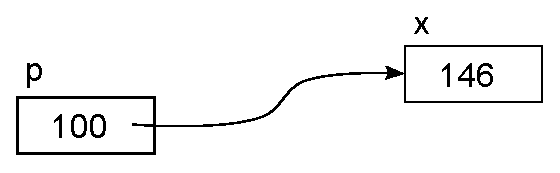
\epsfig{file=figures/arrays/pointers1.eps, height=0.75in}
\end{center}
\caption{แผนภาพ{\wbr}แสดง{\wbr}พอยน์เตอร์ {\ct p}}
\label{fig:array-example-pointer}
\end{figure}

\subsection{การ{\wbr}ประกาศ{\wbr}ชนิด{\wbr}ข้อมูล โอ{\wbr}เปอเรเตอร์ {\ct *} และ {\ct \&}}
วิธีการ{\wbr}ประกาศ{\wbr}และ{\wbr}ใช้{\wbr}ข้อมูล{\wbr}ประเภท{\wbr}นี้{\wbr}ขึ้น{\wbr}กับ{\wbr}ภาษา{\wbr}โปรแกรม{\wbr}ที่{\wbr}ใช้ สำหรับ{\wbr}ภาษา C++
เรา{\wbr}ใช้{\wbr}เครื่องหมาย {\ct *} ใน{\wbr}การ{\wbr}ระบุ{\wbr}ชนิด{\wbr}ข้อมูล กล่าวคือ{\wbr}เรา{\wbr}จะ{\wbr}เขียน{\wbr}

\begin{center}
ชนิด{\wbr}ข้อมูล{\ct *}
\end{center}

เพื่อ{\wbr}ระบุ{\wbr}ว่า{\wbr}เป็น{\wbr}พอยน์เตอร์{\wbr}ไป{\wbr}ยัง{\wbr}ชนิด{\wbr}ข้อมูล{\wbr}ดังกล่าว  ยก{\wbr}ตัวอย่าง{\wbr}เช่น{\wbr}

\begin{center}
{\ct int* p;}
\end{center}

เป็น{\wbr}การ{\wbr}ประกาศ{\wbr}ตัวแปร {\ct p} ที่{\wbr}เป็น{\wbr}พอยน์เตอร์{\wbr}ไป{\wbr}ยัง{\wbr}ข้อมูล{\wbr}ชนิด {\ct int}
ตัวแปร{\wbr}ประเภท{\wbr}พอยน์เตอร์{\wbr}จะ{\wbr}ต้อง{\wbr}อ้าง{\wbr}ถึง{\wbr}ตำแหน่ง{\wbr}ใน{\wbr}หน่วยความจำ{\wbr}
เรา{\wbr}จะ{\wbr}ใช้{\wbr}โอ{\wbr}เปอเรเตอร์{\wbr}แบบ{\wbr}นำหน้า {\ct \&}
ใน{\wbr}การ{\wbr}อ้าง{\wbr}ถึง{\wbr}ตำแหน่ง{\wbr}ใน{\wbr}หน่วยความจำ{\wbr}ของ{\wbr}ตัวแปร{\wbr}หรือ{\wbr}ข้อมูล  ดัง{\wbr}แสดง{\wbr}ใน{\wbr}ตัวอย่าง{\wbr}ด้าน{\wbr}ล่าง{\wbr}

\latintext
\begin{codelist}{C++}{}
int x = 146;
int* p = &x;   // Line 2
\end{codelist}
\thaitext

หลัง{\wbr}การ{\wbr}ทำงาน{\wbr}ใน{\wbr}บรรทัด{\wbr}ที่ 2 ตัวแปร {\ct p} จะ{\wbr}เก็บ{\wbr}ตำแหน่ง{\wbr}ใน{\wbr}หน่วยความจำ{\wbr}ของ{\wbr}ตัวแปร{\wbr}
{\ct x} หรือ{\wbr}เรา{\wbr}จะ{\wbr}กล่าว{\wbr}ว่า {\ct p} ชี้{\wbr}ไป{\wbr}ที่{\wbr}ตัวแปร {\ct x}

ต่อไป{\wbr}ถ้า{\wbr}เรา{\wbr}อ้าง{\wbr}ถึง{\wbr}ตัวแปร {\ct p} เรา{\wbr}จะ{\wbr}หมายถึง ``ตำแหน่ง'' ของ{\wbr}ข้อมูล{\wbr}ใน{\wbr}หน่วยความจำ{\wbr}
ถ้า{\wbr}เรา{\wbr}ต้องการ{\wbr}อ้าง{\wbr}ถึง ``ข้อมูล'' ใน{\wbr}หน่วยความจำ{\wbr}ตำแหน่ง{\wbr}นั้น เรา{\wbr}จะ{\wbr}ใช้{\wbr}โอ{\wbr}เปอเรเตอร์{\wbr}นำหน้า{\wbr}
{\ct *} ยก{\wbr}ตัวอย่าง{\wbr}เช่น{\wbr}ใน{\wbr}โปรแกรม{\wbr}ด้าน{\wbr}ล่าง{\wbr}

\latintext
\begin{codelist}{C++}{}
cout << *p;       // Line 1
*p = 1000;        // Line 2
cout << x;        // Line 3
\end{codelist}
\thaitext

โปรแกรม{\wbr}ใน{\wbr}บรรทัด{\wbr}ที่ 1 จะ{\wbr}พิมพ์{\wbr}ค่า 146 เนื่องจาก{\wbr}ตัวแปร {\ct p} ชี้{\wbr}ไป{\wbr}ที่{\wbr}ตำแหน่ง{\wbr}ของ{\wbr}ตัวแปร{\wbr}
{\ct x} ที่{\wbr}มี{\wbr}ค่า 146 เมื่อ{\wbr}เรา{\wbr}อ้าง{\wbr}ถึง ``ข้อมูล'' ที่{\wbr}ตำแหน่ง{\wbr}ที่ {\ct p} เก็บ{\wbr}อยู่{\wbr}
เรา{\wbr}จึง{\wbr}ได้{\wbr}ค่า{\wbr}เป็น 146

การ{\wbr}อ้าง {\ct *p} หมายถึง{\wbr}ข้อมูล{\wbr}ใน{\wbr}ตำแหน่ง{\wbr}หน่วยความจำ{\wbr}ที่{\wbr}ตัวแปร {\ct p} ชี้{\wbr}อยู่{\wbr}
ดังนั้น{\wbr}โปรแกรม{\wbr}ใน{\wbr}บรรทัด{\wbr}ที่ 2 ก็{\wbr}จะ{\wbr}เป็น{\wbr}การ{\wbr}กำหนด{\wbr}ค่า{\wbr}ให้{\wbr}กับ{\wbr}หน่วยความจำ{\wbr}ที่{\wbr}เดียวกับ{\wbr}ตัวแปร {\ct
  x} ทำ{\wbr}ให้{\wbr}โปรแกรม{\wbr}ใน{\wbr}บรรทัด{\wbr}ที่ 3 พิมพ์{\wbr}ค่า 1000 ออก{\wbr}มา{\wbr}

สังเกต{\wbr}ว่า{\wbr}เครื่องหมาย {\ct *} ใน{\wbr}คำสั่ง {\ct int* p = \&x;} กับ {\ct *p =
  1000;} มี{\wbr}ความหมาย{\wbr}ต่าง{\wbr}กัน ใน{\wbr}ตัวอย่าง{\wbr}แรก{\wbr}เป็น{\wbr}การ{\wbr}ขยาย{\wbr}ชนิด{\wbr}ข้อมูล {\ct int}
เพื่อ{\wbr}ระบุ{\wbr}ชนิด{\wbr}ข้อมูล{\wbr}ว่า{\wbr}เป็น{\wbr}พอยน์เตอร์{\wbr}ไป{\wbr}ยัง{\wbr}จำนวนเต็ม{\wbr}
โดย{\wbr}มี{\wbr}การ{\wbr}กำหนด{\wbr}ค่า{\wbr}เริ่มต้น{\wbr}ด้วย{\wbr}เครื่องหมาย{\wbr}เท่า{\wbr}กับ ใน{\wbr}ตัวอย่าง{\wbr}ที่{\wbr}สอง เครื่องหมาย {\ct *}
เป็น{\wbr}โอ{\wbr}เปอเรเตอร์{\wbr}แบบ{\wbr}นำหน้า ที่{\wbr}กระทำ{\wbr}กับ{\wbr}ตัวแปร {\ct p}  ใน{\wbr}ตัวอย่าง{\wbr}แรก ถ้า{\wbr}เรา{\wbr}ไม่{\wbr}กำหนด{\wbr}ค่า{\wbr}เริ่มต้น{\wbr}ให้{\wbr}กับ{\wbr}พอยน์เตอร์ {\ct p} ทันที{\wbr}เมื่อ{\wbr}ประกาศ โปรแกรม{\wbr}จะ{\wbr}เขียน{\wbr}ได้{\wbr}ดังนี้{\wbr}

\latintext
\begin{codelist}{C++}{}
int* p;
p = &x;
\end{codelist}
\thaitext

โอ{\wbr}เปอเรเตอร์ {\ct *} กับ {\ct \&} เป็น{\wbr}โอ{\wbr}เปอเรเตอร์{\wbr}ที่{\wbr}ทำ{\wbr}หน้าที่{\wbr}ตรงข้าม{\wbr}กัน{\wbr}
ถ้า{\wbr}พิจารณา{\wbr}ตาม{\wbr}แผนภาพ{\wbr}ใน{\wbr}รูป{\wbr}ที่~\ref{fig:array-example-pointer} โอ{\wbr}เปอเรเตอร์
{\ct *} จะ{\wbr}พา{\wbr}เรา{\wbr}ไป{\wbr}ตาม{\wbr}ลูกศร ส่วน {\ct \&} จะ{\wbr}พา{\wbr}เรา{\wbr}ย้อน{\wbr}กลับ{\wbr}

\begin{quiz}{}
นิพจน์ {\ct *(\&x) = 1234;} มี{\wbr}ความหมาย{\wbr}อย่างไร?
\end{quiz}

\begin{quiz}{}
สำหรับ{\wbr}ตัวแปร {\ct x} ที่{\wbr}ประกาศ{\wbr}และ{\wbr}กำหนด{\wbr}ค่า{\wbr}เริ่มต้น{\wbr}ด้วย{\wbr}คำสั่ง {\ct int x = 146;}
นิพจน์ {\ct \&x} หมายถึง{\wbr}ตำแหน่ง{\wbr}ใน{\wbr}หน่วยความจำ{\wbr}ของ {\ct x} นิพจน์ {\ct \&(\&x)} หมายถึง{\wbr}อะไร?
\end{quiz}
\begin{quizans}
นิพจน์{\wbr}ดังกล่าว{\wbr}ไม่{\wbr}มี{\wbr}ความหมาย และ{\wbr}จะ{\wbr}ทำ{\wbr}ให้{\wbr}เกิด{\wbr}ความผิด{\wbr}พลาด{\wbr}ระหว่าง{\wbr}การ{\wbr}คอมไพล์{\wbr}
เพื่อ{\wbr}ความ{\wbr}เข้าใจ{\wbr}ที่{\wbr}ชัดเจน{\wbr}ยิ่ง{\wbr}ขึ้น กรุณา{\wbr}อ่าน{\wbr}ส่วน~\ref{sect:array-lval-rval}
\end{quizans}

ผู้{\wbr}ที่{\wbr}ใช้{\wbr}งาน{\wbr}พอยน์เตอร์{\wbr}นั้น{\wbr}จะ{\wbr}ต้อง{\wbr}ระวัง{\wbr}เป็นพิเศษ{\wbr}ใน{\wbr}การ{\wbr}จัดการ{\wbr}หน่วยความจำ{\wbr}
โดยเฉพาะ{\wbr}เกี่ยวกับ{\wbr}สถานะ{\wbr}ของ{\wbr}หน่วยความจำ{\wbr}ที่{\wbr}พอยน์เตอร์{\wbr}นั้น{\wbr}ชี้{\wbr}ไป{\wbr}
พิจารณา{\wbr}ตัวอย่าง{\wbr}ใน{\wbr}โปรแกรมย่อย{\wbr}ด้าน{\wbr}ล่าง{\wbr}

\latintext
\begin{codelist}{C++}{}
int* crazy(int x)
{
  int y = x + 10;  int* z = &y;
  return z;
}
\end{codelist}
\thaitext

ฟังก์ชัน{\wbr}ดังกล่าว{\wbr}คืน{\wbr}ค่า{\wbr}พอยน์เตอร์{\wbr}ไป{\wbr}ยัง{\wbr}ตัวแปร {\ct y} ซึ่ง{\wbr}เป็น{\wbr}ตัวแปร{\wbr}ภายใน{\wbr}ของ{\wbr}ฟังก์ชัน {\ct
  crazy}
ตัวแปร{\wbr}ประเภท{\wbr}นี้{\wbr}โดย{\wbr}ทั่วไป{\wbr}จะ{\wbr}ถูก{\wbr}เก็บ{\wbr}ใน{\wbr}หน่วยความจำ{\wbr}ที่{\wbr}กัน{\wbr}เนื้อที่{\wbr}ไว้{\wbr}แค่{\wbr}ช่วง{\wbr}ที่{\wbr}ฟังก์ชัน{\wbr}ทำงาน{\wbr}เท่านั้น{\wbr}
เมื่อ{\wbr}ฟังก์ชัน{\wbr}จบ{\wbr}การ{\wbr}ทำงาน{\wbr}ลง หน่วยความจำ{\wbr}ส่วน{\wbr}นี้{\wbr}ก็{\wbr}อาจ{\wbr}จะ{\wbr}ถูก{\wbr}ใช้{\wbr}โดย{\wbr}ตัวแปร{\wbr}อื่น ๆ อย่างไรก็ตาม{\wbr}
พอยน์เตอร์ที่{\wbr}คืน{\wbr}มา{\wbr}ก็{\wbr}ยัง{\wbr}ชี้{\wbr}ไป{\wbr}ที่{\wbr}ตำแหน่ง{\wbr}เดิม{\wbr}ของ{\wbr}ตัวแปร {\ct y} อยู่{\wbr}
ทำ{\wbr}ให้{\wbr}เมื่อ{\wbr}อ่าน{\wbr}เขียน{\wbr}ข้อมูล{\wbr}ใน{\wbr}ตำแหน่ง{\wbr}นั้น{\wbr}
อาจ{\wbr}จะ{\wbr}เกิด{\wbr}ปัญหา{\wbr}ไป{\wbr}เขียน{\wbr}ทับ{\wbr}ข้อมูล{\wbr}ของ{\wbr}ส่วน{\wbr}อื่น{\wbr}ของ{\wbr}โปรแกรม{\wbr}ได้{\wbr}

\subsection{การ{\wbr}จอง{\wbr}หน่วยความจำ: โอ{\wbr}เปอเรเตอร์ {\ct new} และ{\wbr}โอ{\wbr}เปอเรเตอร์ {\ct delete}}
นอกจาก{\wbr}ที่{\wbr}จะ{\wbr}ให้{\wbr}พอยน์เตอร์{\wbr}ชี้{\wbr}ไป{\wbr}ยัง{\wbr}ตัวแปร{\wbr}ต่าง ๆ แล้ว{\wbr}
เรา{\wbr}ยัง{\wbr}สามารถ{\wbr}จอง{\wbr}หน่วยความจำ{\wbr}เพื่อ{\wbr}เก็บ{\wbr}ข้อมูล{\wbr}โดยเฉพาะ{\wbr}ได้{\wbr}ด้วย{\wbr}โอ{\wbr}เปอเรเตอร์ {\ct new}
หน่วยความจำ{\wbr}ที่{\wbr}ขอ{\wbr}จอง{\wbr}มา{\wbr}ได้{\wbr}นี้{\wbr}จะ{\wbr}เป็น{\wbr}หน่วยความจำ{\wbr}ที่{\wbr}ระบบ{\wbr}เชื่อ{\wbr}ว่า{\wbr}ยัง{\wbr}ไม่{\wbr}มี{\wbr}การ{\wbr}ใช้{\wbr}
ทำ{\wbr}ให้{\wbr}เรา{\wbr}สามารถ{\wbr}ใช้เนื้อ{\wbr}ที่{\wbr}เหล่านี้{\wbr}เก็บ{\wbr}ข้อมูล{\wbr}ได้{\wbr}ตาม{\wbr}ต้องการ{\wbr}

โอ{\wbr}เปอเรเตอร์ {\ct new} นอกจาก{\wbr}จะ{\wbr}จอง{\wbr}หน่วยความจำ{\wbr}สำหรับ{\wbr}ข้อมูล{\wbr}แล้ว{\wbr}
ยัง{\wbr}กำหนด{\wbr}ค่า{\wbr}เริ่มต้น{\wbr}ให้{\wbr}กับ{\wbr}ข้อมูล{\wbr}ดังกล่าว{\wbr}ก่อน{\wbr}ที่{\wbr}จะ{\wbr}คืน{\wbr}พอยน์เตอร์{\wbr}กลับ{\wbr}มา{\wbr}

หน่วยความจำ{\wbr}ที่{\wbr}จอง{\wbr}มา{\wbr}นี้ เมื่อ{\wbr}ไม่{\wbr}ใช้{\wbr}แล้ว{\wbr}จะ{\wbr}ต้อง{\wbr}ถูก{\wbr}ปล่อย{\wbr}คืน{\wbr}ให้{\wbr}กับ{\wbr}ระบบ{\wbr}ด้วย{\wbr}โอ{\wbr}เป{\wbr}อร{\wbr}เรเตอร์ {\ct
  delete} เพื่อ{\wbr}เก็บ{\wbr}ไว้{\wbr}จัดสรร{\wbr}ใน{\wbr}ครั้ง{\wbr}ต่อ ๆ ไป  พิจารณา{\wbr}ตัวอย่าง{\wbr}การ{\wbr}ใช้{\wbr}งาน{\wbr}ดังนี้{\wbr}

\latintext
\begin{codelist}{C++}{}
int* p = new int;
int* q = p;           // Line 2
p = new int;          // Line 3
// ...                   Line 4
// ... do something
delete p;
delete q;
\end{codelist}
\thaitext

เมื่อ{\wbr}โปรแกรม{\wbr}ทำงาน{\wbr}ผ่าน{\wbr}บรรทัด{\wbr}ที่ 2 พอยน์เตอร์ {\ct p} และ {\ct q}
จะ{\wbr}ชี้{\wbr}ไป{\wbr}ยัง{\wbr}ตำแหน่ง{\wbr}ที่{\wbr}จอง{\wbr}ไว้{\wbr}ใน{\wbr}หน่วยความจำ{\wbr}เดียวกัน เมื่อ{\wbr}ถึง{\wbr}บรรทัด{\wbr}ที่ 4
ตัวแปร{\wbr}ทั้ง{\wbr}สอง{\wbr}จะ{\wbr}ชี้{\wbr}ไป{\wbr}ยัง{\wbr}หน่วยความจำ{\wbr}คน{\wbr}ละ{\wbr}ที่ เนื่องจาก{\wbr}บรรทัด{\wbr}ที่ 3
เรา{\wbr}ได้{\wbr}จอง{\wbr}หน่วยความจำ{\wbr}ใหม่{\wbr}ให้{\wbr}กับ {\ct p} เมื่อ{\wbr}โปรแกรม{\wbr}ทำงาน{\wbr}เสร็จ เรา{\wbr}ก็{\wbr}จะ{\wbr}สั่ง {\ct
  delete} เพื่อให้{\wbr}ระบบ{\wbr}คืน{\wbr}ค่า{\wbr}หน่วยความจำ{\wbr}ที่{\wbr}จอง{\wbr}ไว้{\wbr}ทั้ง{\wbr}สอง{\wbr}หน่วย{\wbr}

พิจารณา{\wbr}ตัวอย่าง{\wbr}โปรแกรม{\wbr}ด้าน{\wbr}ล่าง{\wbr}

\latintext
\begin{codelist}{C++}{}
int c = 0;
for(int i = 0; i < N; ++i) {
  int* p = new int;
  p = c + i;
  c = p;
}
\end{codelist}
\thaitext

\begin{quiz}{}
โปรแกรม{\wbr}ข้างต้น{\wbr}ทำงาน{\wbr}อะไร  ถ้า{\wbr}ตัวแปร {\ct N} มี{\wbr}ค่า{\wbr}มาก ๆ โปรแกรม{\wbr}ดังกล่าว{\wbr}จะ{\wbr}ทำ{\wbr}ให้{\wbr}เกิด{\wbr}อะไร{\wbr}ขึ้น{\wbr}
\end{quiz}

ความ{\wbr}สามารถ{\wbr}ใน{\wbr}การ{\wbr}จอง{\wbr}หน่วยความจำ{\wbr}เมื่อ{\wbr}โปรแกรม{\wbr}ทำงาน{\wbr}นี้{\wbr}เป็น{\wbr}สิ่ง{\wbr}ที่{\wbr}จำเป็น{\wbr}มาก{\wbr}ใน{\wbr}การ{\wbr}พัฒนา{\wbr}โครงสร้าง{\wbr}ข้อมูล{\wbr}ที่{\wbr}ซับซ้อน{\wbr}ขึ้น{\wbr}ต่อไป{\wbr}
อย่างไรก็ตาม ถ้า{\wbr}เรา{\wbr}ไม่{\wbr}ระมัดระวัง{\wbr}พอ{\wbr}และ{\wbr}ไม่{\wbr}คืน{\wbr}หน่วยความจำ{\wbr}ที่{\wbr}จอง{\wbr}ไว้{\wbr}เมื่อ{\wbr}เลิก{\wbr}อ้าง{\wbr}ถึง{\wbr}แล้ว{\wbr}
เรา{\wbr}อาจ{\wbr}จะ{\wbr}พบ{\wbr}ปัญหา{\wbr}โปรแกรม{\wbr}ใช้{\wbr}หน่วยความจำ{\wbr}มาก{\wbr}เกิน{\wbr}ไป{\wbr}เนื่องจาก{\wbr}มี{\wbr}การ{\wbr}รั่วไหล{\wbr}ของ{\wbr}การ{\wbr}ใช้{\wbr}งาน{\wbr}หน่วยความจำ{\wbr}ก็ได้{\wbr}
(เรียก{\wbr}ว่า memory leak)

ใน{\wbr}ภาษา C++
เรา{\wbr}สามารถ{\wbr}ซ่อน{\wbr}การ{\wbr}ทำงาน{\wbr}ของ{\wbr}โครงสร้าง{\wbr}ข้อมูล{\wbr}รวม{\wbr}ถึง{\wbr}การ{\wbr}จอง{\wbr}และ{\wbr}คืน{\wbr}หน่วยความจำ{\wbr}ไว้{\wbr}ภายใน{\wbr}ค{\wbr}ลา{\wbr}ส
ถ้า{\wbr}พัฒนา{\wbr}อย่าง{\wbr}ถูก{\wbr}วิธี จะ{\wbr}ช่วย{\wbr}ลด{\wbr}ปัญหา{\wbr}หน่วยความจำ{\wbr}รั่วไหล{\wbr}ได้{\wbr}

\subsection{พอยน์เตอร์{\wbr}ว่าง}
นอกจาก{\wbr}เรา{\wbr}จะ{\wbr}กำหนด{\wbr}ค่า{\wbr}ใหัตัว{\wbr}แปร{\wbr}พอยน์เตอร์{\wbr}ชี้{\wbr}ไป{\wbr}ที่{\wbr}ตำแหน่ง{\wbr}ต่าง ๆ
ใน{\wbr}หน่วยความจำ{\wbr}โดย{\wbr}ใช้{\wbr}โอ{\wbr}เปอเรเตอร์ {\ct\&} แล้ว{\wbr}
เรา{\wbr}ยัง{\wbr}สามารถ{\wbr}กำหนด{\wbr}ให้{\wbr}ตัวแปร{\wbr}พอยน์เตอร์{\wbr}มี{\wbr}สถานะ{\wbr}เป็น ``ไม่{\wbr}ได้{\wbr}ชี้{\wbr}ไป{\wbr}ที่ไหน''
ได้{\wbr}โดย{\wbr}การ{\wbr}กำหนด{\wbr}ค่า {\ct 0} ให้{\wbr}กับ{\wbr}ตัวแปร{\wbr}พอยน์เตอร์{\wbr}นั้น\footnote{ใน{\wbr}มาตรฐาน C++11
  มี{\wbr}การ{\wbr}นิยาม{\wbr}ค่าคงที่ {\ct nullptr}
  เพื่อ{\wbr}ใช้{\wbr}แทน{\wbr}พอยน์เตอร์{\wbr}ว่าง{\wbr}เพื่อ{\wbr}แก้{\wbr}ปัญหา{\wbr}การ{\wbr}ใช้{\wbr}ค่าคงที่{\wbr}ซ้ำซ้อน อย่างไรก็ตาม{\wbr}
  เพื่อให้{\wbr}หนังสือ{\wbr}นี้{\wbr}ใช้{\wbr}งาน{\wbr}ได้{\wbr}กับ{\wbr}คอม{\wbr}ไพ{\wbr}เลอร์{\wbr}ที่{\wbr}ยัง{\wbr}ไม่{\wbr}ปรับ{\wbr}รุ่น{\wbr}ให้{\wbr}ทัน{\wbr}มาตรฐาน{\wbr}ใหม่{\wbr}นี้{\wbr}
  เรา{\wbr}จะ{\wbr}ยัง{\wbr}ใช้{\wbr}ค่าคงที่ {\ct 0} เพื่อ{\wbr}แทน{\wbr}พอยน์เตอร์{\wbr}ว่าง{\wbr}อยู่ ถ้า{\wbr}ผู้อ่าน{\wbr}ใช้{\wbr}คอม{\wbr}ไพ{\wbr}เลอร์{\wbr}รุ่น{\wbr}ใหม่{\wbr}แล้ว{\wbr}
  ขอ{\wbr}แนะนำ{\wbr}ให้{\wbr}ใช้ {\ct nullptr} แทน {\ct 0}}\footnote{ใน{\wbr}ภาษา C นิยม{\wbr}ใช้{\wbr}ค่าคงที่{\wbr}
  {\ct NULL} ที่{\wbr}นิยาม{\wbr}ไว้{\wbr}ใน{\wbr}ไฟล์{\wbr}หัว{\wbr}มาตรฐาน อย่างไรก็ตาม เรา{\wbr}สามารถ{\wbr}ใช้{\wbr}ค่าคงที่ 0 ใน{\wbr}
  C++ ได้{\wbr}เลย} พอยน์เตอร์ดังกล่าว{\wbr}เรียก{\wbr}ว่า{\wbr}เป็น{\em พอยน์เตอร์ว่าง} ({\em null
  pointer})

พอยน์เตอร์ที่{\wbr}มี{\wbr}ค่า{\wbr}เป็น{\wbr}พอยน์เตอร์{\wbr}ว่าง{\wbr}นี้ ใน{\wbr}ภาษา C++
ไม่{\wbr}ได้{\wbr}ทำงาน{\wbr}แตกต่าง{\wbr}จาก{\wbr}พอยน์เตอร์{\wbr}ธรรมดา{\wbr}เท่าใด{\wbr}นัก นั่น{\wbr}คือ{\wbr}
โปรแกรม{\wbr}สามารถ{\wbr}เรียกหา{\wbr}ค่า{\wbr}ที่{\wbr}ชี้{\wbr}โดย{\wbr}พอยน์เตอร์{\wbr}ดังกล่าว{\wbr}ได้{\wbr}
ผลลัพธ์{\wbr}ที่{\wbr}ได้{\wbr}ขึ้น{\wbr}กับ{\wbr}คอม{\wbr}ไพ{\wbr}เลอร์{\wbr}และ{\wbr}ระบบปฏิบัติการ{\wbr}ที่{\wbr}ใช้ แต่{\wbr}โดย{\wbr}ทั่วไป{\wbr}การ{\wbr}เรียก{\wbr}อ่าน{\wbr}ค่า{\wbr}ตำแหน่ง{\wbr}ที่ 0
มักจะ{\wbr}ถูก{\wbr}ป้องกัน{\wbr}ไว้{\wbr}ด้วย{\wbr}ระบบปฏิบัติการ ทำ{\wbr}ให้{\wbr}โปรแกรม{\wbr}ที่{\wbr}เรียก{\wbr}ใช้{\wbr}ดังกล่าว crash ได้{\wbr}เป็นต้น{\wbr}
อย่างไรก็ตาม ภาษา C/C++ รับประกัน{\wbr}ว่า{\wbr}พอยน์เตอร์{\wbr}ว่าง{\wbr}สอง{\wbr}ตัว{\wbr}จะ{\wbr}เปรียบเทียบ{\wbr}ได้{\wbr}เท่า{\wbr}กัน{\wbr}
ถึงแม้{\wbr}จะ{\wbr}เป็น{\wbr}พอยน์เตอร์{\wbr}คน{\wbr}ละ{\wbr}ชนิด{\wbr}ก็ตาม{\wbr}

\subsection{ชนิด{\wbr}ข้อมูล{\wbr}แบบ {\ct void} และ{\wbr}พอยน์เตอร์{\wbr}ไป{\wbr}ยัง {\ct void}}

ชนิด{\wbr}ข้อมูล {\ct void} เป็น{\wbr}ชนิด{\wbr}ข้อมูล{\wbr}พิเศษ{\wbr}ที่{\wbr}ไม่{\wbr}มี{\wbr}ข้อมูล{\wbr}ใด{\wbr}เป็น{\wbr}สมาชิก{\wbr}
การ{\wbr}ประกาศ{\wbr}ว่า{\wbr}ฟังก์ชัน{\wbr}คืน{\wbr}ค่า{\wbr}เป็น{\wbr}ข้อมูล{\wbr}ชนิด{\wbr}นี้{\wbr}คือ{\wbr}การ{\wbr}ประกาศ{\wbr}ว่า{\wbr}ฟังก์ชัน{\wbr}ดังกล่าว{\wbr}ไม่{\wbr}คืน{\wbr}ค่า{\wbr}
นอกจาก{\wbr}เรา{\wbr}จะ{\wbr}ใช้ {\ct void} เพื่อ{\wbr}ระบุ{\wbr}ฟังก์ชัน{\wbr}แล้ว พอยน์เตอร์ไป{\wbr}ยัง {\ct void}
(ชนิด{\wbr}ข้อมูล {\ct void*})
แทน{\wbr}พอยน์เตอร์{\wbr}ที่{\wbr}ชี้{\wbr}ไป{\wbr}ยัง{\wbr}ตำแหน่ง{\wbr}ใน{\wbr}หน่วยความจำ{\wbr}ที่{\wbr}เรา{\wbr}ไม่{\wbr}สนใจ{\wbr}ว่า{\wbr}จะ{\wbr}เป็น{\wbr}ข้อมูล{\wbr}ชนิด{\wbr}ใด{\wbr}
เรา{\wbr}สามารถ{\wbr}กำหนด{\wbr}ค่า{\wbr}พอยน์เตอร์{\wbr}ไป{\wbr}ยัง{\wbr}ข้อมูล{\wbr}ใด ๆ ให้{\wbr}กับ{\wbr}พอยน์เตอร์{\wbr}ประเภท {\ct void*} ได้{\wbr}
และ{\wbr}พอยน์เตอร์{\wbr}ประเภท {\ct void*} ก็{\wbr}สามารถ{\wbr}ถูก{\wbr}แปลง (cast) เป็น{\wbr}พอยน์เตอร์{\wbr}ประเภท{\wbr}อื่น{\wbr}
ๆ ได้ อย่างไรก็ตาม{\wbr}การ{\wbr}แปลง{\wbr}ใน{\wbr}ลักษณะ{\wbr}นี้{\wbr}
ถ้า{\wbr}ไม่{\wbr}ระวัง{\wbr}อาจ{\wbr}ก่อ{\wbr}ให้{\wbr}เกิด{\wbr}ข้อผิดพลาด{\wbr}ระหว่าง{\wbr}การ{\wbr}ทำงาน{\wbr}ได้{\wbr}


\subsection{พอยน์เตอร์กับ{\wbr}การ{\wbr}ส่ง{\wbr}พารามิเตอร์}
เรา{\wbr}สามารถ{\wbr}ใช้{\wbr}พอยน์เตอร์{\wbr}เพื่อ{\wbr}ส่ง{\wbr}ค่า{\wbr}ผ่าน{\wbr}พารามิเตอร์{\wbr}ใน{\wbr}ลักษณะ{\wbr}เดียวกับ{\wbr}การ{\wbr}ส่ง{\wbr}แบบ pass by
reference ได้ พิจารณา{\wbr}ฟังก์ชัน{\wbr}ด้าน{\wbr}ล่าง{\wbr}ที่{\wbr}สลับ{\wbr}ค่า{\wbr}ใน{\wbr}ตัวแปร{\wbr}สอง{\wbr}ตัว{\wbr}

\latintext
\begin{codelist}{C++}{}
void swap1(int& a, int& b)
{
  int t = a;
  a = b;
  b = t;
}
\end{codelist}
\thaitext

ฟังก์ชัน{\wbr}นี้{\wbr}ทำงาน{\wbr}ได้{\wbr}ตาม{\wbr}ที่{\wbr}เรา{\wbr}ต้องการ เนื่องจาก{\wbr}ชนิด{\wbr}ข้อมูล{\wbr}ของ{\wbr}พารามิเตอร์ {\ct a} และ {\ct
  b} คือ {\ct int\&} ฟังก์ชัน{\wbr}ดัง{\wbr}ด้าน{\wbr}ล่าง{\wbr}จะ{\wbr}ไม่{\wbr}สามารถ{\wbr}สลับ{\wbr}ค่า{\wbr}ใน{\wbr}ตัวแปร{\wbr}ที่{\wbr}ส่ง{\wbr}มา{\wbr}ได้{\wbr}
แม้ว่า{\wbr}ค่า{\wbr}ใน{\wbr}ตัวแปร {\ct a} และ {\ct b} จะ{\wbr}เปลี่ยน{\wbr}ใน{\wbr}ฟังก์ชัน{\wbr}ก็ตาม{\wbr}
เพราะว่า{\wbr}การ{\wbr}ส่ง{\wbr}ค่า{\wbr}โดย{\wbr}ปกติ{\wbr}จะ{\wbr}เป็น{\wbr}การ{\wbr}ส่ง{\wbr}แบบ pass by value

\latintext
\begin{codelist}{C++}{}
void swap2(int a, int b)    // broken
{
  int t = a;
  a = b;
  b = t;
}
\end{codelist}
\thaitext

อย่างไรก็ตาม เนื่องจาก{\wbr}เรา{\wbr}ต้องการ{\wbr}เปลี่ยนแปลง{\wbr}ค่า{\wbr}ของ{\wbr}อาร์กิวเมนท์{\wbr}ที่{\wbr}ส่ง{\wbr}มา{\wbr}ให้{\wbr}กับ{\wbr}ฟังก์ชัน{\wbr}
เรา{\wbr}จำเป็น{\wbr}ต้อง{\wbr}อ้าง{\wbr}ถึง{\wbr}ตำแหน่ง{\wbr}ของ{\wbr}อาร์กิวเมนท์{\wbr}นั้น ด้าน{\wbr}ล่าง{\wbr}เป็น{\wbr}ฟังก์ชัน {\ct swap3}
ที่{\wbr}เขียน{\wbr}โดย{\wbr}ใช้{\wbr}พอยน์เตอร์

\latintext
\begin{codelist}{C++}{}
void swap3(int* a, int* b)
{
  int t = *a;
  *a = *b;
  *b = t;
}
\end{codelist}
\thaitext

เนื่องจาก{\wbr}ฟังก์ชัน {\ct swap3} รับ{\wbr}อาร์กิวเมนท์{\wbr}เป็น{\wbr}พอยน์เตอร์
การ{\wbr}เรียก{\wbr}ใช้{\wbr}งาน{\wbr}ก็{\wbr}จะ{\wbr}ยุ่งยาก{\wbr}ขึ้น{\wbr}เล็กน้อย ดัง{\wbr}แสดง{\wbr}ใน{\wbr}โปรแกรม{\wbr}ด้าน{\wbr}ล่าง{\wbr}

\latintext
\begin{codelist}{C++}{}
int x = 100;
int y = 1000;
swap3(&x, &y);
\end{codelist}
\thaitext

รูป~\ref{fig:array-swap} แสดง{\wbr}การ{\wbr}ชี้{\wbr}ของ{\wbr}พอยน์เตอร์{\wbr}ใน{\wbr}การ{\wbr}เรียก{\wbr}ใช้{\wbr}งาน{\wbr}ฟังก์ชัน {\ct swap3}

\begin{figure}
\begin{center}
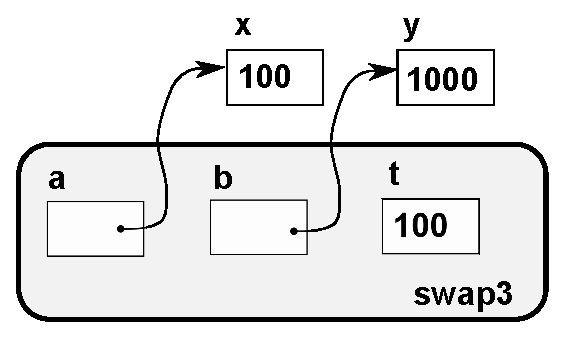
\epsfig{file=figures/arrays/swap3.eps, height=1.2in}
\end{center}
\caption{พอยน์เตอร์{\wbr}ต่าง ๆ ใน{\wbr}การ{\wbr}เรียก{\wbr}ใช้{\wbr}ฟังก์ชัน {\ct swap3}}
\label{fig:array-swap}
\end{figure}


\begin{quiz}{}
ฟังก์ชัน {\ct swap1} และ {\ct swap3} แม้{\wbr}มี{\wbr}การ{\wbr}ทำงาน{\wbr}ที่{\wbr}เหมือน{\wbr}กัน การ{\wbr}เรียก{\wbr}ใช้{\wbr}งาน{\wbr}
{\ct swap3} นั้น{\wbr}ดู{\wbr}ยุ่งยาก{\wbr}กว่า อย่างไรก็ตาม{\wbr}
มี{\wbr}บาง{\wbr}กรณี{\wbr}ที่{\wbr}การ{\wbr}ประกาศ{\wbr}พารามิเตอร์{\wbr}ที่{\wbr}ต้องการ{\wbr}แก้ไข{\wbr}ด้วย{\wbr}พอยน์เตอร์{\wbr}ทำ{\wbr}ให้{\wbr}เรา{\wbr}มี{\wbr}อิสระ{\wbr}ใน{\wbr}การ{\wbr}เรียก{\wbr}ใช้{\wbr}งาน{\wbr}มาก{\wbr}กว่า กรณี{\wbr}นั้น{\wbr}คือ{\wbr}อะไร?
\end{quiz}
\begin{quizans}
ใน{\wbr}กรณี{\wbr}ของ{\wbr}การ{\wbr}ส่ง{\wbr}ตัวแปร{\wbr}แบบ pass by reference
ทาง{\wbr}ฝั่ง{\wbr}ผู้{\wbr}เรียก{\wbr}ใช้{\wbr}ฟังก์ชัน{\wbr}จำเป็น{\wbr}ต้อง{\wbr}มี{\wbr}ตัวแปร{\wbr}เพื่อ{\wbr}ส่ง{\wbr}มา{\wbr}ยัง{\wbr}พารามิเตอร์{\wbr}นี้{\wbr}
แต่{\wbr}ใน{\wbr}กรณี{\wbr}ของ{\wbr}การ{\wbr}ส่ง{\wbr}แบบ{\wbr}พอยน์เตอร์
พารามิเตอร์{\wbr}ดังกล่าว{\wbr}จะ{\wbr}เป็น{\wbr}พารามิเตอร์{\wbr}ที่{\wbr}สามารถ{\wbr}ละ{\wbr}เอา{\wbr}ไว้{\wbr}ได้{\wbr}โดย{\wbr}ส่ง พอยน์เตอร์ว่าง {\ct 0}
มา{\wbr}แทน ดังนั้น ใน{\wbr}การ{\wbr}ประกาศ{\wbr}พารามิเตอร์ ถ้า{\wbr}พารามิเตอร์{\wbr}ใด จำเป็น{\wbr}ต้อง{\wbr}มี{\wbr}ตัวแปร{\wbr}มา{\wbr}รับ{\wbr}ค่า{\wbr}
เรา{\wbr}ควร{\wbr}จะ{\wbr}ใช้{\wbr}การ{\wbr}ประกาศ{\wbr}แบบ pass by reference
ถ้า{\wbr}พารามิเตอร์{\wbr}นั้น{\wbr}ไม่{\wbr}จำเป็น{\wbr}ต้อง{\wbr}มี{\wbr}อยู่จริง{\wbr}ใน{\wbr}บาง{\wbr}กรณี{\wbr}
เรา{\wbr}ก็{\wbr}ควร{\wbr}จะ{\wbr}ประกาศ{\wbr}รับ{\wbr}พารามิเตอร์{\wbr}ด้วย{\wbr}พอยน์เตอร์{\wbr}แทน{\wbr}
\end{quizans}

\subsection{การ{\wbr}คำนวณ{\wbr}กับ{\wbr}พอยน์เตอร์}
\label{sect:array-pointer-arith}

เรา{\wbr}สามารถ{\wbr}ดำเนินการ{\wbr}เชิง{\wbr}ตัวเลข{\wbr}กับ{\wbr}พอยน์เตอร์{\wbr}ได้ ปกติ{\wbr}พอยน์เตอร์{\wbr}สำหรับ{\wbr}ชนิด{\wbr}ข้อมูล{\wbr}ใด ๆ
ก็{\wbr}จะ{\wbr}ใช้{\wbr}ชี้{\wbr}ไป{\wbr}ยัง{\wbr}ตำแหน่ง{\wbr}ใน{\wbr}หน่วยความจำ{\wbr}ของ{\wbr}ข้อมูล{\wbr}ชนิด{\wbr}นั้น พิจารณา{\wbr}ตัวอย่าง{\wbr}โปรแกรม{\wbr}ด้าน{\wbr}ล่าง{\wbr}

\latintext
\begin{codelist}{C++}{}
int a[5];
char b[10];
int* p = &a[3];
char* q = &b[0];
\end{codelist}
\thaitext

ถ้า{\wbr}เรา{\wbr}สมมติ{\wbr}ว่า{\wbr}ข้อมูล{\wbr}ประเภท {\ct int} ใช้เนื้อ{\wbr}ที่ 4 ไบท์ใน{\wbr}การ{\wbr}จัด{\wbr}เก็บ{\wbr}ใน{\wbr}หน่วยความจำ และ{\wbr}
{\ct char} ใช้เนื้อ{\wbr}ที่ 1 ไบท์ใน{\wbr}การ{\wbr}จัด{\wbr}เก็บ ตัวแปร{\wbr}ต่าง ๆ
จะ{\wbr}อยู่{\wbr}ใน{\wbr}หน่วยความจำ{\wbr}ดัง{\wbr}ใน{\wbr}รูป{\wbr}ที่~\ref{fig:array-array-pointer-arith}

\begin{figure}
\begin{center}
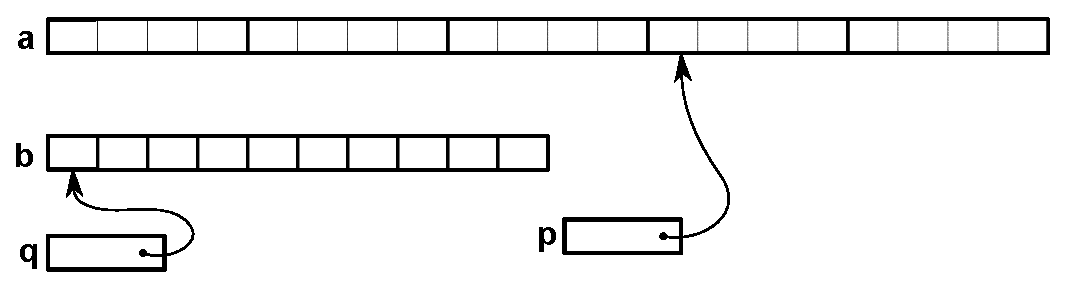
\epsfig{file=figures/arrays/pointer-arith.eps, height=1.2in}
\end{center}
\caption{พอยน์เตอร์ที่{\wbr}ชี้{\wbr}ที่{\wbr}ตำแหน่ง{\wbr}ต่าง ๆ ใน{\wbr}อาร์เรย์}
\label{fig:array-array-pointer-arith}
\end{figure}

เนื่องจาก{\wbr}พอยน์เตอร์{\wbr}ถูก{\wbr}นิยาม{\wbr}เทียบ{\wbr}กับ{\wbr}ชนิด{\wbr}ข้อมูล{\wbr}ที่{\wbr}ชี้{\wbr}ไป{\wbr}
ดังนั้น{\wbr}จึง{\wbr}ไม่{\wbr}แปลก{\wbr}อะไร{\wbr}ถ้า{\wbr}เมื่อ{\wbr}เรา{\wbr}เพิ่ม{\wbr}หรือ{\wbr}ลด{\wbr}ค่า{\wbr}ของ{\wbr}พอยน์เตอร์{\wbr}นั้น{\wbr}ด้วย{\wbr}จำนวนเต็ม{\wbr}
เรา{\wbr}จะ{\wbr}หมายถึง{\wbr}ตำแหน่ง{\wbr}ของ{\wbr}ข้อมูล{\wbr}ชนิด{\wbr}นั้น{\wbr}ตัว{\wbr}ถัด ๆ ไป หรือ{\wbr}ตัว{\wbr}ก่อน ๆ หน้า ยก{\wbr}ตัวอย่าง{\wbr}เช่น {\ct
  p+1} เป็น{\wbr}พอยน์เตอร์{\wbr}ที่{\wbr}ชี้{\wbr}ไป{\wbr}ที่ {\ct a[4]} และ {\ct q+1} เป็น{\wbr}พอยน์เตอร์{\wbr}ที่{\wbr}ชี้{\wbr}ไป{\wbr}ที่{\wbr}
{\ct b[1]}

สังเกต{\wbr}ว่า{\wbr}เรา{\wbr}บวก 1 เข้า{\wbr}กับ {\ct p} เพื่อ{\wbr}เลื่อน{\wbr}จาก {\ct a[3]} ไป{\wbr}ยัง {\ct a[4]}
ถึงแม้ว่า{\wbr}ตำแหน่ง{\wbr}ใน{\wbr}หน่วยความจำ{\wbr}ของ {\ct a[3]} และ {\ct a[4]} จะ{\wbr}ต่าง{\wbr}กัน 4
ตำแหน่ง{\wbr}ก็ตาม{\wbr}

นอกจาก{\wbr}การ{\wbr}บวก{\wbr}และ{\wbr}ลบ{\wbr}ด้วย{\wbr}จำนวนเต็ม{\wbr}แล้ว{\wbr}
เรา{\wbr}ยัง{\wbr}สามารถ{\wbr}นำ{\wbr}พอยน์เตอร์{\wbr}ที่{\wbr}ชี้{\wbr}ไป{\wbr}ยัง{\wbr}ข้อมูล{\wbr}ชนิด{\wbr}เดียวกัน{\wbr}มา{\wbr}ลบ{\wbr}กัน{\wbr}ได้{\wbr}ด้วย{\wbr}

\begin{quiz}{}
พิจารณา{\wbr}ตัวแปร {\ct int* r = \&a[1]} และ {\ct int* s = \&a[4]} นิพจน์ {\ct s
  - r} มี{\wbr}ค่า{\wbr}เป็น{\wbr}เท่าใด?
\end{quiz}

\subsection{อาร์เรย์{\wbr}และ{\wbr}พอยน์เตอร์{\wbr}ใน{\wbr}ภาษา C/C++}
\label{sect:array-array-pointer-c}

สังเกต{\wbr}ว่า{\wbr}จาก{\wbr}ส่วน{\wbr}ที่~\ref{sect:array-pointer-arith}
เรา{\wbr}สามารถ{\wbr}ใช้{\wbr}พอยน์เตอร์{\wbr}ใน{\wbr}การ{\wbr}ประมวลผล{\wbr}ข้อมูล{\wbr}ใน{\wbr}อาร์เรย์{\wbr}ได้{\wbr}
ยก{\wbr}ตัวอย่าง{\wbr}เช่น{\wbr}ฟังก์ชัน{\wbr}ใน{\wbr}โปรแกรม{\wbr}ที่~\ref{code:array-sum-using-pointer}
ที่{\wbr}หา{\wbr}ผลรวม{\wbr}ของ{\wbr}ข้อมูล{\wbr}ใน{\wbr}รายการ{\wbr}

\latintext
\begin{codelist}{C++}{caption={\thaitext ฟังก์ชัน{\wbr}ที่{\wbr}หา{\wbr}ผลรวม{\wbr}ของ{\wbr}ข้อมูล{\wbr}ใน{\wbr}รายการ{\wbr}โดย{\wbr}ใช้{\wbr}พอยน์เตอร์{\wbr}วิ่ง{\wbr}ไป{\wbr}ใน{\wbr}อาร์เรย์\latintext},label=code:array-sum-using-pointer}
int sum1(int list[], int size)            
{
  int s = 0;
  int* p = &list[0];
  for(int i = 0; i < size; ++i) {
    s += *p;
    ++p;
  }
  return s;
}
\end{codelist}
\thaitext

\begin{quiz}{}
โปรแกรม~\ref{code:array-sum-using-pointer} ปรับ{\wbr}ค่า{\wbr}พอยน์เตอร์ {\ct p}
ให้{\wbr}ชี้{\wbr}ไป{\wbr}ยัง{\wbr}ข้อมูล{\wbr}ต่าง ๆ ใน{\wbr}อาร์เรย์ ให้{\wbr}แก้{\wbr}ฟังก์ชัน {\ct sum1} ให้{\wbr}ทำงาน{\wbr}ได้{\wbr}เหมือน{\wbr}เดิม{\wbr}
โดย{\wbr}ให้{\wbr}พอยน์เตอร์ {\ct p} มี{\wbr}ค่าคงที่{\wbr}โดย{\wbr}ชี้{\wbr}อยู่{\wbr}ที่{\wbr}ตำแหน่ง{\wbr}ของ {\ct list[0]} ตลอดเวลา{\wbr}
\end{quiz}

สังเกต{\wbr}ว่า{\wbr}ใน{\wbr}โปรแกรม~\ref{code:array-sum-using-pointer} เรา{\wbr}ยัง{\wbr}ใช้{\wbr}ดัชนี {\ct i}
ใน{\wbr}การ{\wbr}วน{\wbr}รอบ{\wbr}อยู่ อย่างไรก็ตาม ยัง{\wbr}มี{\wbr}อีก{\wbr}รูปแบบ{\wbr}ใน{\wbr}การ{\wbr}เขียน{\wbr}ที่{\wbr}อาจ{\wbr}จะ{\wbr}ดู{\wbr}กระ{\wbr}ทัด{\wbr}รัด{\wbr}กว่า{\wbr}
ดัง{\wbr}แสดง{\wbr}ใน{\wbr}โปรแกรม~\ref{code:array-sum-using-end-pointer}

\latintext
\begin{codelist}{C++}{caption={\thaitext ฟังก์ชัน{\wbr}ที่{\wbr}หา{\wbr}ผลรวม{\wbr}ของ{\wbr}ข้อมูล{\wbr}ใน{\wbr}รายการ{\wbr}โดย{\wbr}ใช้{\wbr}พอยน์เตอร์{\wbr}วิ่ง{\wbr}ไป{\wbr}ใน{\wbr}อาร์เรย์ อีก{\wbr}แบบ{\wbr}หนึ่ง\latintext},label=code:array-sum-using-end-pointer}
int sum2(int list[], int size)
{
  int s = 0;
  int* p = &list[0];             // Line 4
  int* end = &list[size];        // Line 5
  while(p != end) {
    c += *p;
    ++p;
  }
  return s;
}
\end{codelist}
\thaitext

สังเกต{\wbr}ว่า{\wbr}ใน{\wbr}โปรแกรม~\ref{code:array-sum-using-end-pointer} ตัวแปร {\ct
  end} อาจ{\wbr}จะ{\wbr}ชี้{\wbr}ออก{\wbr}ไป{\wbr}นอก{\wbr}ขอบเขต{\wbr}ของ{\wbr}อาร์เรย์{\wbr}ได้ ใน{\wbr}กรณี{\wbr}นี้ ภาษา C++
รับประกัน{\wbr}ว่า{\wbr}พอยน์เตอร์{\wbr}ที่{\wbr}ชี้{\wbr}ไป{\wbr}ที่{\wbr}ข้อมูล{\wbr}ที่{\wbr}เกิน{\wbr}อาร์เรย์{\wbr}ไป 1 หน่วย จะ{\wbr}ยัง{\wbr}สามารถ{\wbr}ใช้{\wbr}งาน{\wbr}ได้{\wbr}
เพื่อให้{\wbr}การ{\wbr}เขียน{\wbr}โปรแกรม{\wbr}ใน{\wbr}ลักษณะ{\wbr}นี้{\wbr}ไม่{\wbr}เกิด{\wbr}ข้อผิดพลาด อย่างไรก็ตาม{\wbr}
การ{\wbr}อ้าง{\wbr}พอยน์เตอร์{\wbr}ออก{\wbr}ไป{\wbr}ยัง{\wbr}ตำแหน่ง{\wbr}ที่อยู่{\wbr}ก่อนหน้า{\wbr}ข้อมูล{\wbr}ตัวแปร{\wbr}ของ{\wbr}อาร์เรย์
หรือ{\wbr}ตำแหน่ง{\wbr}ที่{\wbr}เกิน{\wbr}กว่า{\wbr}ข้อมูล{\wbr}ตัว{\wbr}สุดท้าย{\wbr}มาก{\wbr}กว่า 1 ตำแหน่ง{\wbr}นั้น{\wbr}
ระบบ{\wbr}จะ{\wbr}ไม่{\wbr}รับประกัน{\wbr}ว่า{\wbr}จะ{\wbr}สามารถ{\wbr}ทำ{\wbr}ได้{\wbr}

ใน{\wbr}ภาษา C++ นอกจาก{\wbr}ที่{\wbr}เรา{\wbr}จะ{\wbr}นำ{\wbr}พอยน์เตอร์{\wbr}ไป{\wbr}ชี้{\wbr}ที่{\wbr}อาร์เรย์{\wbr}เพื่อ{\wbr}ประมวลผล{\wbr}ได้{\wbr}แล้ว{\wbr}
เรา{\wbr}ยัง{\wbr}สามารถ{\wbr}นำ{\wbr}อาร์เรย์{\wbr}และ{\wbr}พอยน์เตอร์{\wbr}มา{\wbr}ใช้{\wbr}สลับ{\wbr}กัน{\wbr}ไป{\wbr}มา{\wbr}ได้{\wbr}ใน{\wbr}อีก{\wbr}หลาย ๆ กรณี{\wbr}
เรา{\wbr}จะ{\wbr}เริ่ม{\wbr}จาก{\wbr}กรณี{\wbr}ที่{\wbr}ใช้{\wbr}อาร์เรย์{\wbr}ใน{\wbr}รูป{\wbr}ของ{\wbr}พอยน์เตอร์{\wbr}ก่อน{\wbr}

สำหรับ{\wbr}อาร์เรย์{\wbr}ใด ๆ ถ้า{\wbr}เรา{\wbr}อ้าง{\wbr}ถึง{\wbr}อาร์เรย์{\wbr}โดย{\wbr}ไม่{\wbr}ระบุ{\wbr}ดัชนี{\wbr}
เรา{\wbr}จะ{\wbr}ได้{\wbr}ค่า{\wbr}เป็น{\wbr}ตำแหน่ง{\wbr}ของ{\wbr}ข้อมูล{\wbr}ตัว{\wbr}แรก{\wbr}ใน{\wbr}อาร์เรย์ ดังนั้น{\wbr}บรรทัด{\wbr}ที่ 4 และ 5
ใน{\wbr}โปรแกรม~\ref{code:array-sum-using-end-pointer} สามารถ{\wbr}แก้{\wbr}เป็น{\wbr}ดัง{\wbr}ด้าน{\wbr}ล่าง{\wbr}ได้{\wbr}

\latintext
\begin{codelist}{C++}{}
  int* p = list;                 // Line 4
  int* end = list + size;        // Line 5
\end{codelist}
\thaitext

อย่างไรก็ตาม ถึงแม้ว่า{\wbr}เรา{\wbr}จะ{\wbr}อ้าง{\wbr}ตัวแปร{\wbr}อาร์เรย์{\wbr}เป็น{\wbr}พอยน์เตอร์{\wbr}ได้{\wbr}
เรา{\wbr}จะ{\wbr}ไม่{\wbr}สามารถ{\wbr}กำหนด{\wbr}ค่า{\wbr}ให้{\wbr}กับ{\wbr}มัน{\wbr}ได้ โปรแกรม{\wbr}ด้าน{\wbr}ล่าง{\wbr}จะ{\wbr}คอมไพล์{\wbr}ไม่{\wbr}ผ่าน{\wbr}ถ้า{\wbr}ตัวแปร {\ct
  list} เป็น{\wbr}อาร์เรย์ แต่{\wbr}ถ้า {\ct list} เป็น{\wbr}พอยน์เตอร์{\wbr}จะ{\wbr}สามารถ{\wbr}ทำ{\wbr}ได้{\wbr}
(ใน{\wbr}ภาษา{\wbr}เชิง{\wbr}เทคนิค เรา{\wbr}จะ{\wbr}กล่าว{\wbr}ว่า{\wbr}นิพจน์ {\ct list} ไม่{\wbr}มี L-value ผู้{\wbr}ที่{\wbr}สนใจ{\wbr}สามารถ{\wbr}
อ่าน{\wbr}เพิ่มเติม{\wbr}ได้{\wbr}ใน{\wbr}ส่วน~\ref{sect:array-lval-rval})

\latintext
\begin{codelist}{C++}{}
  list = list + 1;              // does not compile
\end{codelist}
\thaitext

\begin{quiz}{}
โปรแกรมเมอร์{\wbr}ที่{\wbr}เขียน{\wbr}คำสั่ง {\ct list = list + 1; }  ใน{\wbr}ตัวอย่าง{\wbr}ข้างต้น ต้องการ{\wbr}จะ{\wbr}ทำ{\wbr}อะไร?
\end{quiz}

ใน{\wbr}กรณี{\wbr}ของ{\wbr}อาร์เรย์{\wbr}หลาย{\wbr}มิติ การ{\wbr}อ้าง{\wbr}ถึง{\wbr}อาร์เรย์{\wbr}ด้วย{\wbr}ชื่อ{\wbr}ก็{\wbr}จะ{\wbr}ได้{\wbr}ผลลัพธ์{\wbr}เป็น{\wbr}พอยน์เตอร์{\wbr}เช่นกัน{\wbr}
โดย{\wbr}พอยน์เตอร์{\wbr}ที่{\wbr}ได้{\wbr}จะ{\wbr}ชี้{\wbr}ไป{\wbr}ยัง{\wbr}ตำแหน่ง{\wbr}ของ{\wbr}ข้อมูล{\wbr}ตัว{\wbr}แรก{\wbr}ที่{\wbr}สอดคล้อง{\wbr}กับ{\wbr}การ{\wbr}อ้าง{\wbr}ถึง{\wbr}ขณะนั้น{\wbr}
และ{\wbr}มี{\wbr}ชนิด{\wbr}ข้อมูล{\wbr}สอดคล้อง{\wbr}กับ{\wbr}ระดับ{\wbr}ของ{\wbr}การ{\wbr}อ้าง{\wbr}ถึง ยก{\wbr}ตัวอย่าง{\wbr}เช่น ถ้า{\wbr}เรา{\wbr}ประกาศ{\wbr}อาร์เรย์ {\ct
  int a[100][200];} การ{\wbr}อ้าง{\wbr}ถึง {\ct a} จะ{\wbr}เป็น{\wbr}พอยน์เตอร์{\wbr}ชี้{\wbr}ไป{\wbr}ที่{\wbr}ตำแหน่ง{\wbr}ของ {\ct
  a[0][0]} และ{\wbr}มี{\wbr}ชนิด{\wbr}ข้อมูล{\wbr}เป็น {\ct int**} (พอยน์เตอร์ไป{\wbr}ยัง{\wbr}พอยน์เตอร์{\wbr}ไป{\wbr}ยัง {\ct
  int}) ส่วน {\ct a[10]} จะ{\wbr}เป็น{\wbr}พอยน์เตอร์{\wbr}ชนิด {\ct int*} ชี้{\wbr}ไป{\wbr}ที่{\wbr}ตำแหน่ง{\wbr}ของ {\ct
  a[10][0]} เป็นต้น{\wbr}

เช่นเดียวกับ{\wbr}ใน{\wbr}ตัวอย่าง{\wbr}ข้างต้น ทั้ง {\ct a} และ {\ct a[10]} เป็น{\wbr}นิพจน์{\wbr}ที่{\wbr}มี{\wbr}ค่า{\wbr}
แต่{\wbr}ไม่{\wbr}สามารถ{\wbr}กำหนด{\wbr}ค่า{\wbr}ให้{\wbr}ได้ เนื่องจาก{\wbr}เรา{\wbr}ไม่{\wbr}มี{\wbr}ตัวแปร{\wbr}ใน{\wbr}หน่วยความจำ{\wbr}จริง ๆ ที่{\wbr}เก็บ{\wbr}ค่า{\wbr}เหล่านี้{\wbr}
(นั่น{\wbr}คือ {\ct a} และ {\ct a[10]} ไม่{\wbr}มี L-value)

ใน{\wbr}มุมกลับ{\wbr}กัน เรา{\wbr}สามารถ{\wbr}ใช้{\wbr}พอยน์เตอร์{\wbr}ใน{\wbr}ลักษณะ{\wbr}เดียวกับ{\wbr}อาร์เรย์{\wbr}ได้ กล่าวคือ ถ้า {\ct p}
เป็น{\wbr}พอยน์เตอร์ การ{\wbr}อ้าง {\ct p[0]} จะ{\wbr}มี{\wbr}ความหมาย{\wbr}เดียวกับ {\ct *p} และ{\wbr}การ{\wbr}อ้าง{\wbr}
{\ct p[10]} จะ{\wbr}มี{\wbr}ความหมาย{\wbr}เดียวกับ {\ct *(p + 10)} ดังนั้น{\wbr}หลาย ๆ
ครั้ง{\wbr}เรา{\wbr}จะ{\wbr}พบ{\wbr}ว่า{\wbr}ฟังก์ชัน{\wbr}ที่{\wbr}รับ{\wbr}ค่า{\wbr}เป็น{\wbr}อาร์เรย์
แต่{\wbr}กลับ{\wbr}ประกาศ{\wbr}ว่า{\wbr}รับ{\wbr}พารามิเตอร์{\wbr}เป็น{\wbr}พอยน์เตอร์{\wbr}เพื่อ{\wbr}ความ{\wbr}สะดวก{\wbr}ใน{\wbr}การ{\wbr}ใช้{\wbr}งาน{\wbr}

\begin{quiz}{}
ถ้า{\wbr}ใน{\wbr}โปรแกรม เรา{\wbr}มี{\wbr}ความ{\wbr}จะ{\wbr}เป็น{\wbr}ต้อง{\wbr}เลื่อน{\wbr}ดัชนี{\wbr}ทั้งหมด{\wbr}ของ{\wbr}อาร์เรย์ {\ct list} ลง{\wbr}หนึ่ง{\wbr}
หลาย ๆ ครั้ง{\wbr}
เรา{\wbr}จะ{\wbr}ความ{\wbr}สามารถ{\wbr}ใน{\wbr}การ{\wbr}สลับ{\wbr}เปลี่ยน{\wbr}ระหว่าง{\wbr}อาร์เรย์{\wbr}และ{\wbr}พอยน์เตอร์{\wbr}เพื่อ{\wbr}ดำเนินการ{\wbr}ดังกล่าว{\wbr}ได้{\wbr}อย่างไร{\wbr}
\end{quiz}

การ{\wbr}ใช้{\wbr}งาน{\wbr}พอยน์เตอร์{\wbr}ใน{\wbr}รูปแบบ{\wbr}ของ{\wbr}อาร์เรย์{\wbr}เพิ่ม{\wbr}ความ{\wbr}สะดวก{\wbr}ใน{\wbr}การ{\wbr}ใช้{\wbr}งาน{\wbr}อาร์เรย์{\wbr}ที่{\wbr}เรา{\wbr}ต้อง{\wbr}จอง{\wbr}หน่วยความจำ{\wbr}เอง{\wbr}
โดยมาก{\wbr}จะ{\wbr}เป็น{\wbr}อาร์เรย์{\wbr}ที่{\wbr}เรา{\wbr}ไม่{\wbr}ทราบ{\wbr}ขนาด{\wbr}ก่อน{\wbr}ถึง{\wbr}เวลา{\wbr}ใช้{\wbr}งาน หรือ{\wbr}กระทั่ง{\wbr}เป็น{\wbr}อาร์เรย์{\wbr}ที่{\wbr}มี{\wbr}ขนาด{\wbr}เปลี่ยน{\wbr}ไป{\wbr}มา{\wbr}ได้{\wbr}

โอ{\wbr}เปอเรเตอร์ {\ct new} และ {\ct delete}
สามารถ{\wbr}ใช้{\wbr}เพื่อ{\wbr}จอง{\wbr}หน่วยความจำ{\wbr}แบบ{\wbr}อาร์เรย์{\wbr}ได้ โดย{\wbr}รูปแบบ{\wbr}ใน{\wbr}การ{\wbr}ใช้{\wbr}งาน{\wbr}เป็น{\wbr}ดังนี้{\wbr}

\begin{center}
{\ct new} ชนิด{\wbr}ข้อมูล[จำนวน{\wbr}ข้อมูล] \\
{\ct delete []} ตัวแปร{\wbr}
\end{center}

สังเกต{\wbr}ว่า{\wbr}เรา{\wbr}ระบุ{\wbr}จำนวน{\wbr}ช่อง{\wbr}ของ{\wbr}ข้อมูล{\wbr}ที่{\wbr}ต้องการ{\wbr}ใช้{\wbr}ใน{\wbr}โอ{\wbr}เปอเรเตอร์ {\ct new}
และ{\wbr}ใส่{\wbr}เครื่องหมาย {\ct []} เมื่อ{\wbr}ใช้{\wbr}โอ{\wbr}เปอเรเตอร์ {\ct delete}
เพื่อ{\wbr}ระบุ{\wbr}ว่า{\wbr}เป็น{\wbr}การ{\wbr}ทำลาย{\wbr}อาร์เรย์ ดัง{\wbr}ตัวอย่าง{\wbr}ด้าน{\wbr}ล่าง{\wbr}

\latintext
\begin{codelist}{C++}{}
  int* a = new int[100];

  for(int i = 0; i < 100; ++i) 
    a[i] = i;
  // ...

  delete [] a;
\end{codelist}
\thaitext

สังเกต{\wbr}ว่า{\wbr}เรา{\wbr}ใช้{\wbr}งาน{\wbr}ตัวแปร{\wbr}พอยน์เตอร์ {\ct a} ใน{\wbr}ลักษณะ{\wbr}เดียวกับ{\wbr}อาร์เรย์ ข้อ{\wbr}ควร{\wbr}ระวัง{\wbr}ก็{\wbr}คือ{\wbr}
ถ้า{\wbr}เรา{\wbr}เรียก{\wbr}โอ{\wbr}เปอเรเตอร์ {\ct new} แบบ{\wbr}อาร์เรย์ เมื่อ{\wbr}เรา{\wbr}เรียก {\ct delete}
เรา{\wbr}จะ{\wbr}ต้อง{\wbr}ระบุ {\ct []} ด้วย{\wbr}ทุก{\wbr}ครั้ง ไม่{\wbr}เช่นนั้น{\wbr}โอ{\wbr}เปอเรเตอร์ delete
อาจ{\wbr}ทำงาน{\wbr}ผิดพลาด{\wbr}ได้{\wbr}

\subsection{แนว{\wbr}คิด{\wbr}เกี่ยวกับ L-value และ R-value $\star$}
\label{sect:array-lval-rval}

พิจารณา{\wbr}คำสั่ง{\wbr}กำหนด{\wbr}ค่า{\wbr}ด้าน{\wbr}ล่าง{\wbr}

\latintext
\begin{codelist}{C++}{}
x = x + 1;
\end{codelist}
\thaitext

ใน{\wbr}คำสั่ง{\wbr}ดังกล่าว{\wbr}เรา{\wbr}กล่าว{\wbr}ถึง{\wbr}ตัวแปร {\ct x} สอง{\wbr}ครั้ง{\wbr}
ถ้า{\wbr}พิจารณา{\wbr}ให้{\wbr}ดี{\wbr}เรา{\wbr}จะ{\wbr}พบ{\wbr}ว่าความ{\wbr}หมาย{\wbr}ของ{\wbr}การ{\wbr}กล่าว{\wbr}ถึง{\wbr}ทั้ง{\wbr}สอง{\wbr}ครั้งนั้น{\wbr}แตกต่าง{\wbr}กัน{\wbr}

\begin{itemize}
\item เมื่อ{\wbr}เรา{\wbr}กล่าว{\wbr}ถึง {\ct x} ใน{\wbr}ด้าน{\wbr}ซ้าย{\wbr}ของ{\wbr}เครื่องหมาย{\wbr}กำหนด{\wbr}ค่า{\wbr}
  สิ่ง{\wbr}ที่{\wbr}เรา{\wbr}ต้องการ{\wbr}จาก{\wbr}ตัวแปร {\ct x} คือ{\wbr}ตำแหน่ง{\wbr}ใน{\wbr}หน่วยความจำ{\wbr}
  เพื่อให้{\wbr}ระบบ{\wbr}สามารถ{\wbr}เก็บ{\wbr}ผลลัพธ์{\wbr}ได้{\wbr}
\item สำหรับ{\wbr}การ{\wbr}กล่าว{\wbr}ถึง{\wbr}ตัวแปร {\ct x} ใน{\wbr}ด้าน{\wbr}ขวา{\wbr}ของ{\wbr}เครื่องหมาย{\wbr}กำหนด{\wbr}ค่า{\wbr}นั้น{\wbr}
  สิ่ง{\wbr}ที่{\wbr}เรา{\wbr}ต้องการ{\wbr}ได้{\wbr}คือ{\wbr}ค่า{\wbr}ของ{\wbr}ข้อมูล{\wbr}ที่{\wbr}เก็บ{\wbr}ใน{\wbr}ตัวแปร {\ct x}
\end{itemize}

เรา{\wbr}จะ{\wbr}เรียก ``ความหมาย'' ของ{\wbr}นิพจน์{\wbr}ใด ๆ เมื่อ{\wbr}อยู่{\wbr}ด้าน{\wbr}ขวา{\wbr}ของ{\wbr}เครื่องหมาย{\wbr}กำหนด{\wbr}ค่า{\wbr}
ว่า{\wbr}เป็น R-value ของ{\wbr}นิพจน์{\wbr}นั้น ซึ่ง{\wbr}ความหมาย{\wbr}นี้ จะ{\wbr}สอดคล้อง{\wbr}กับ{\wbr}ค่า{\wbr}ของ{\wbr}นิพจน์{\wbr}นั้น ๆ
ใน{\wbr}ทาง{\wbr}กลับ{\wbr}กัน L-value ก็{\wbr}เป็น ``ความหมาย'' ของ{\wbr}นิพจน์{\wbr}นั้น{\wbr}
เมื่อ{\wbr}อยู่{\wbr}ด้าน{\wbr}ซ้าย{\wbr}ของ{\wbr}เครื่องหมาย{\wbr}กำหนด{\wbr}ค่า สังเกต{\wbr}ว่า{\wbr}บาง{\wbr}นิพจน์{\wbr}จะ{\wbr}ไม่{\wbr}มี{\wbr}ค่า L-value
นั่น{\wbr}หมายความ{\wbr}ว่า{\wbr}เรา{\wbr}ไม่{\wbr}สามารถ{\wbr}ใช้{\wbr}นิพจน์{\wbr}นั้น{\wbr}ใน{\wbr}ด้าน{\wbr}ซ้าย{\wbr}ของ{\wbr}เครื่องหมาย{\wbr}กำหนด{\wbr}ค่า{\wbr}ได้ นั่น{\wbr}คือ{\wbr}
กำหนด{\wbr}ค่า{\wbr}ไม่{\wbr}ได้{\wbr}นั่นเอง{\wbr}

\section{แบบฝึกหัด}

\begin{enumerate}
\item เขียน{\wbr}โปรแกรม{\wbr}ลำ{\wbr}ลอง{\wbr}สำหรับ{\wbr}การ{\wbr}แทรก{\wbr}ข้อมูล{\wbr}ใน{\wbr}รายการ{\wbr}
\end{enumerate}
